\clearpage
\section{Target-dependent equation selection}
\label{sec:equation-selection}
The preceding policies choose seeds and source rows, but each retained seed
can produce several identities. A third model selects identities for the
requested targets before Kira performs modular independence elimination.
This choice can reduce the system that Kira processes, provided that the
saved algebraic work exceeds the cost of making the choice. We therefore
measure equation preparation and the complete reduction with the model
included~\cite{Kira3,KiraEquationSelectionData}.

\subsection{The equations and their training labels}
Let $\mathcal T$ be the set of requested integral indices. An identity
generated from seed $\boldsymbol\sigma$ and derivative or
Lorentz-invariance operator $o$ has the form
\begin{equation}
 E_{\boldsymbol\sigma,o}:\qquad
 \sum_{\boldsymbol a\in A_{\boldsymbol\sigma,o}}
 c_{\boldsymbol\sigma,o,\boldsymbol a}(\boldsymbol x,d)
 I_{\boldsymbol a}=0 .
 \label{eq:equation-selection-identity}
\end{equation}
Here $A_{\boldsymbol\sigma,o}$ is the set of integral indices that occur
in the identity and $c_{\boldsymbol\sigma,o,\boldsymbol a}$ is the
coefficient of $I_{\boldsymbol a}$. The variables $\boldsymbol x$ and
$d$ retain their definitions as the kinematic parameters and integration
dimension. The operator index distinguishes the several identities from
one seed, so the third policy can retain only part of a seed's output.

We first run native Kira reductions on training families and record the
integral supports of the equations retained in the final regenerated
system. An integral support is the set of indices with nonzero
coefficients after combining repeated terms at the finite-field selection
point. If $\mathcal S_{\rm native}$ is the collection of these supports,
the training label is
\begin{equation}
 y_{\boldsymbol\sigma,o}
 =\mathbf 1\!\left[
  \operatorname{supp}(E_{\boldsymbol\sigma,o})
  \in\mathcal S_{\rm native}\right].
 \label{eq:equation-selection-label}
\end{equation}
The indicator $\mathbf 1$ equals one when the condition holds and zero
otherwise. Several equations can have the same support and different
coefficients, so this label describes support membership in the recorded
selection. It supplies a conservative training proxy and does not establish
a necessary or smallest equation set.

The training collection contains 74,692 candidate equations, with
5,978 positive labels, from ten target batches in six physical profiles.
These profiles comprise two-loop sunrise and double-box integrals and
three-loop vacuum integrals. We keep three additional profiles for
validation and eight for testing. The held-out tests also include a
three-loop ladder topology absent from the training and validation
collections. Each profile fixes rational masses and kinematic invariants,
while the reductions retain symbolic dependence on $d$.

\subsection{Features and the learned probability}
The model receives 23 numerical features that describe the family,
the target set, the seed and the generated equation. These features include
the numbers of loops and external momenta, the number of integral indices,
the target count, positive propagator powers, numerator powers, sector
membership, the operator index and the equation's integral terms.
For example, the distance from a seed to the targets is
\begin{equation}
 \delta(\boldsymbol\sigma,\mathcal T)
 =\min_{\boldsymbol a\in\mathcal T}
   \sum_{i=1}^{N}|\sigma_i-a_i| ,
 \label{eq:equation-selection-distance}
\end{equation}
where $N$ is the number of expressions in the integral family.
The model also uses differences between the seed's dot or numerator
counts and the largest corresponding counts in the target set and
in the same sector. These quantities describe which equations lie near
the requested part of the integral-index lattice.

We fit a classification tree using weighted impurity reduction,
with equal total weight for each training profile~\cite{CART1984}.
A sequence of feature comparisons leads to a leaf, which stores
\begin{equation}
 p_{\boldsymbol\sigma,o}
 =\frac{n_+ + 1/2}{n_{\rm leaf}+1},
 \qquad
 E_{\boldsymbol\sigma,o}\ \hbox{is retained if}\
 p_{\boldsymbol\sigma,o}\geq\tau .
 \label{eq:equation-selection-probability}
\end{equation}
Here $n_+$ is the number of positive training rows in that leaf,
$n_{\rm leaf}$ is its total number of training rows and $\tau$ is
the retention threshold. The fitted tree has 233 nodes and a maximum
depth of eight. Each accepted split leaves at least 24 rows in each
child. The score is a smoothed empirical frequency of the recorded
label, and its numerical value has no separate calibration guarantee.

Training the tree takes 2.75 seconds after the native examples have
been collected. This time excludes the generation of training reductions.
We retain one additional diagnostic field for coefficient-text length,
but exclude it from the decisions because equivalent coefficient
expressions can have different printed lengths. The saved model and
its compiled evaluator give identical probabilities for 18,754 candidates
in the implementation checks.

\subsection{Native integration and the cost of a decision}
Kira constructs a candidate identity before the model first scores it.
The retained identities then enter native modular equation processing.
Symmetry identities and preferred-basis relations continue through their
existing paths. The model scores the IBP and Lorentz-invariance identities
at the generation interface; it does not replace Kira's later algebraic
independence checks.

Several operators share one seed, so we calculate their common
seed-to-target features once. We also store each seed--operator decision.
When Kira later requests the same identity, a stored omission allows the
generation code to skip rebuilding its coefficients. A retained identity
is regenerated through the native code. The tree also calculates an equation feature only when a comparison
on its chosen path needs that feature. Propagator and numerator counts
come directly from the native integral ordering. These saved decisions avoid
repeated predictions and remove part of the repeated equation generation.
Exact comparisons check that the implementation changes preserve the
decision features, probabilities, masks and reduction results.

After reduction, we require every target to lie in the prescribed master
basis. An incomplete filtered attempt triggers an unfiltered native
attempt, followed by an enlarged native seed range when necessary.
The benchmark additionally compares every exported rational coefficient
with an independently stored native reference. The application interface
requires the master basis and can operate without reference target
coefficients; we check these application outputs separately after the
reducer returns.

\subsection{Validation and held-out comparisons}
We select thresholds using complete reduction times on the three
validation profiles. A topology uses the learned filter in the automatic
route only when its validation time ratio is below $0.98$; other
topologies retain native equation choices. The test also includes a
forced learned filter and a deterministic distance filter using
Eq.~\eqref{eq:equation-selection-distance}. Validation selects each
filter's threshold before the test runs, and the saved hashes fix the
model, integration and test protocol.

The test contains fourteen target batches from eight physical profiles.
Each sunrise batch contains 21 targets; the other profiles use batches
of 32 and 128 targets. Five alternating repetitions compare native choices,
the forced learned filter, the distance filter and the automatic route,
giving 280 complete workflows. All four arms use the same compiled
binary, with native choices switching off the three learned policies.
Each time includes preparation, loading,
predictions, equation generation, exact algebra, output checks and all
failed attempts before fallback. The experiment driver is already running when timing begins; Kira process startup and model loading are included. Creation of the independent references
and compression of the evidence files lie outside this timer.

Equation preparation includes generation with modular processing,
equation selection, modular solving and equation regeneration.
It therefore measures the full preparation affected by the filter.
We report median times within each batch and geometric ratios with equal
weight for each physical profile. Descriptive intervals resample these
eight profiles 10,000 times. These intervals describe this finite set of
profiles and do not establish performance for arbitrary multiloop families.

\subsection{Results and scope}
The validation route is double box: off, sunrise: learned at $\tau=0.001$, vacuum3: learned at $\tau=0.0001$. Other topologies use native equation choices. The forced learned filter uses $\tau=0.001$, while the distance filter retains seeds with $\delta\leq 4$. These choices remain fixed throughout the held-out tests.

All 280 complete workflows reproduce their native reference coefficients. The independent audit checks 91,240 coefficient pairs, including 1,931 distinct expression pairs, by exact rational simplification in $d$. The workflows contain 40 failed filtered attempts before successful fallback, and their times include these attempts. Native median complete times range from 0.785 to 5.880 seconds across the fourteen batches.

The forced learned filter has a complete-time ratio of 1.080, with descriptive interval $[0.976,1.220]$. Its equation-preparation ratio is 1.053, with descriptive interval $[0.904,1.224]$. The generated-equation ratio is 0.769, and the selected-equation ratio is 0.985. All ratios use the matched native control, so a value below one indicates a lower measured cost.

The distance filter has a complete-time ratio of 1.016, with descriptive interval $[0.994,1.040]$. Its equation-preparation ratio is 1.089, with descriptive interval $[1.035,1.144]$. The generated-equation ratio is 1.000, and the selected-equation ratio is 1.000. All ratios use the matched native control, so a value below one indicates a lower measured cost.

The automatic route has a complete-time ratio of 1.098, with descriptive interval $[0.981,1.259]$. Its equation-preparation ratio is 1.062, with descriptive interval $[0.896,1.261]$. The generated-equation ratio is 0.849, and the selected-equation ratio is 1.000. All ratios use the matched native control, so a value below one indicates a lower measured cost.

The automatic route does not lower the aggregate complete time in this test. Equation-count changes therefore do not establish an overall runtime gain.

\begin{figure}[htbp]
 \centering
 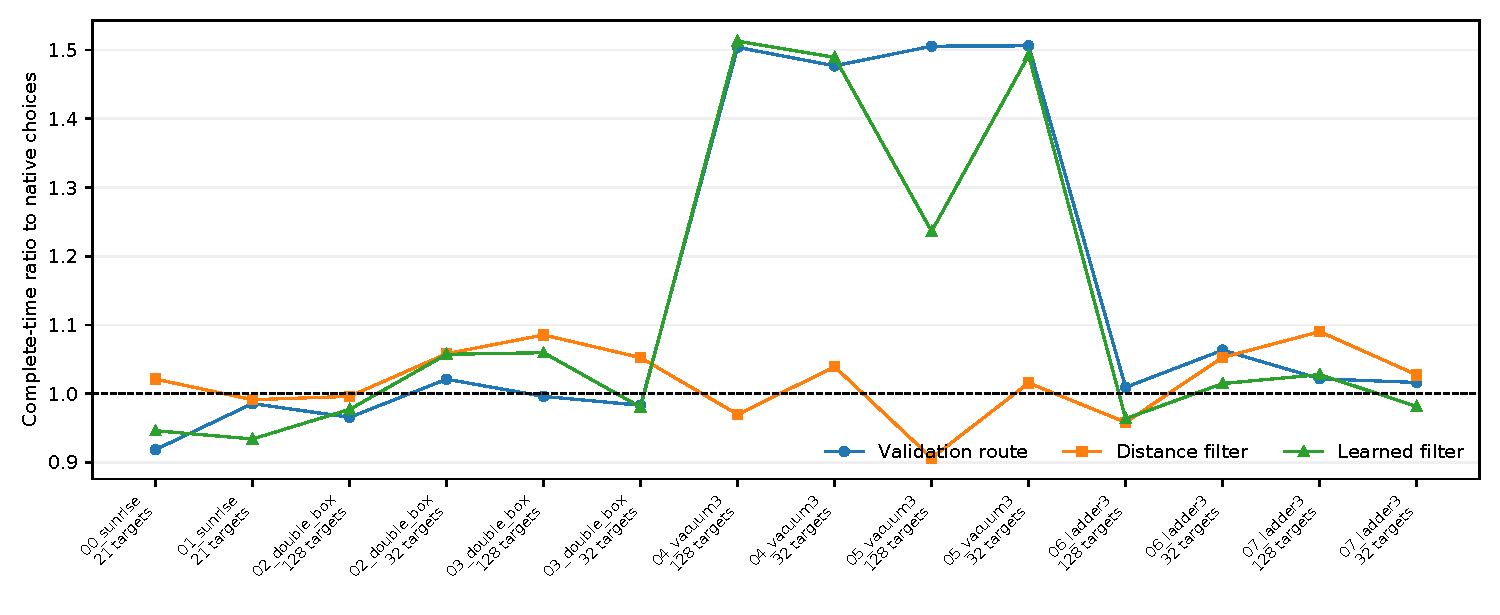
\includegraphics[width=\textwidth]{figures/equation_complete_times.pdf}
 \caption{Median complete-time ratios for the fourteen held-out batches.
 Each point uses five repetitions and includes checks and fallback.
 The dashed line is the native control.}
 \label{fig:equation-complete}
\end{figure}
\begin{figure}[htbp]
 \centering
 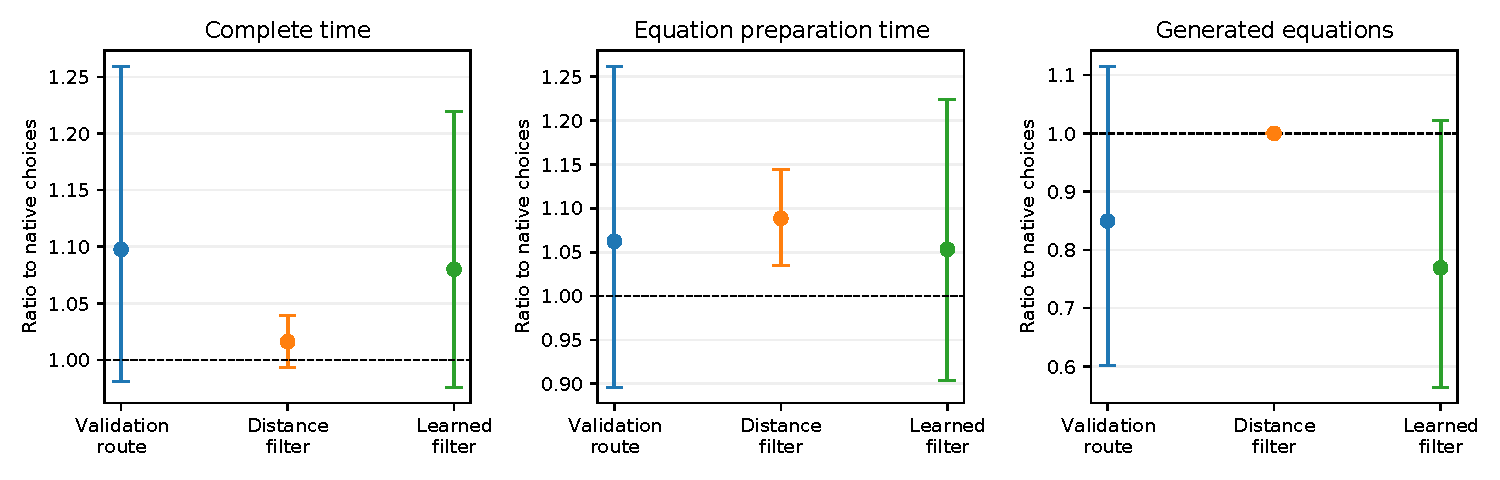
\includegraphics[width=\textwidth]{figures/equation_aggregate_costs.pdf}
 \caption{Profile-weighted geometric ratios of complete time, equation
 preparation time and generated-equation count. Bars show descriptive
 intervals from resampling the eight physical profiles.}
 \label{fig:equation-aggregate}
\end{figure}

After freezing the model, we also collect 77,246 held-out candidate labels, with 6,932 positive labels. At the forced learned threshold, precision is 11.33\% and recall is 95.63\%, with mean squared probability error 0.0621. These quantities measure agreement with the native support-membership proxy. Exact coefficient comparisons measure the validity of the resulting reductions.

\begin{figure}[htbp]
 \centering
 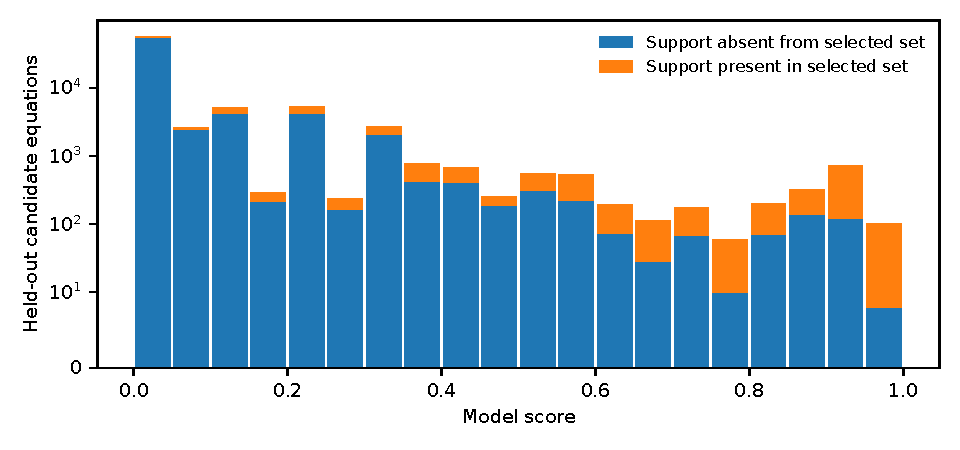
\includegraphics[width=.78\textwidth]{figures/equation_label_scores.pdf}
 \caption{Held-out model scores grouped by the native support-membership
 label. The vertical scale is linear near zero and logarithmic above ten
 equations. The labels describe selected supports rather than necessary
 equations.}
 \label{fig:equation-labels}
\end{figure}

A further 48 complete workflows test the equation route together with the existing row policy and with both existing policies on four profiles. Adding the equation route gives a complete-time ratio of 1.165 to the row-only configuration and 1.184 to the configuration with both earlier models. These comparisons use three repetitions and retain all fallback costs. All pass the reference checks. Eight application runs also pass exact coefficient comparisons after execution with reference coefficients withheld from the reducer.

The early full-feature implementation and subsequent feature-sharing implementations remain in the evidence collection, including their slower results. The final comparison uses the frozen implementation selected before held-out testing. Its performance depends on target size, topology and the cost of generating and reducing the retained equations. The experiment covers physical two- and three-loop reductions at fixed rational kinematics with symbolic $d$; it does not establish gains on arbitrary higher-loop or fully multiscale problems~\cite{KiraEquationSelectionData}.
\FloatBarrier

\subsection{The domain selected before testing}
Validation enables the equation model for the sunrise and three-loop vacuum topologies. This identifies four of the eight test profiles before any test timing is available. On these profiles, the automatic route has a complete-time ratio of 1.194, with descriptive interval $[0.951,1.498]$. Its equation-preparation ratio is 1.078, with descriptive interval $[0.765,1.519]$. The corresponding generated-equation ratio is 0.722.

For sunrise profiles, the automatic complete-time ratio is 0.951 and the preparation ratio is 0.765. For vacuum3 profiles, the automatic complete-time ratio is 1.498 and the preparation ratio is 1.519. For double box profiles, the automatic complete-time ratio is 0.991 and the preparation ratio is 0.988. For ladder3 profiles, the automatic complete-time ratio is 1.027 and the preparation ratio is 1.110. The double-box and ladder routes retain native equation choices, so differences between their automatic and native timings mainly reflect repeated-run variation and routing overhead. The all-profile comparison remains the primary result; these fixed-domain results state where the learned filter was active.



\clearpage
\subsection{Restricted deployment and fresh confirmation}
The broad test exposes incomplete equation filters in the new vacuum
profiles. Their native fallback retains exact results and adds cost.
We therefore fix a restricted deployment using the same trained tree.
It enables the equation filter at $\tau=0.001$ for the recorded
21-target sunrise batches and retains native equation choices for
other topologies and target sets. The broader test supplies development
evidence for this deployment revision.

Each supported batch contains the top-sector scalar integral and its
one-dot and one-numerator variants, together with the corresponding
integrals in the three two-propagator sectors. This gives 21 targets
whose index vectors are fixed in the deployment definition.
We reserve six additional mass and momentum profiles before running
their reductions. None of these profiles occurs in the preceding
training, validation or broad-test sets. Their squared masses and
external invariant are fixed rational numbers, while $d$ remains symbolic.
The tree, threshold, target domain and new profile definitions are
fixed before this confirmation begins.

Nine alternating repetitions compare the learned filter, native choices
and the previously selected distance control in each profile. These
162 complete workflows use the same timing and exact-check rules
as the preceding test, including every failed attempt.

The learned filter has a complete-time ratio of 0.994, with descriptive interval $[0.991,0.997]$ and an equation-preparation ratio of 0.785, with descriptive interval $[0.776,0.794]$. Its generated-equation ratio is 0.414, and its selected-equation ratio is 1.000. The distance control has a complete-time ratio of 1.003, with descriptive interval $[1.000,1.006]$.

The complete-time interval remains below one for these six profiles, supporting a measured gain within the restricted domain.

A further 36 workflows compare the existing seed and row policies with the configuration that also includes the equation filter. Adding the third model gives a complete-time ratio of 1.317, with descriptive interval $[1.296,1.337]$ and a preparation ratio of 1.151, with descriptive interval $[1.136,1.168]$ to the two-model configuration. This comparison uses three repetitions in each of the six profiles.

All 162 main workflows, 36 composition workflows and six basis-only applications pass the independent exact audit, which checks 7,582 coefficient pairs. The 204 workflows include 54 failed attempts. The six applications receive the prescribed masters without reference target coefficients, and their outputs pass coefficient comparisons after execution.

Native median complete times range from 0.692 to 0.709 seconds in these six profiles. The geometric mean preparation fraction of native complete time is 3.29\%. This small fraction explains why the reduction in preparation time produces a smaller change in complete time. The main confirmation has zero failed attempts; all 54 failed attempts in its extended audit arise in the composition comparisons.

\begin{figure}[htbp]
 \centering
 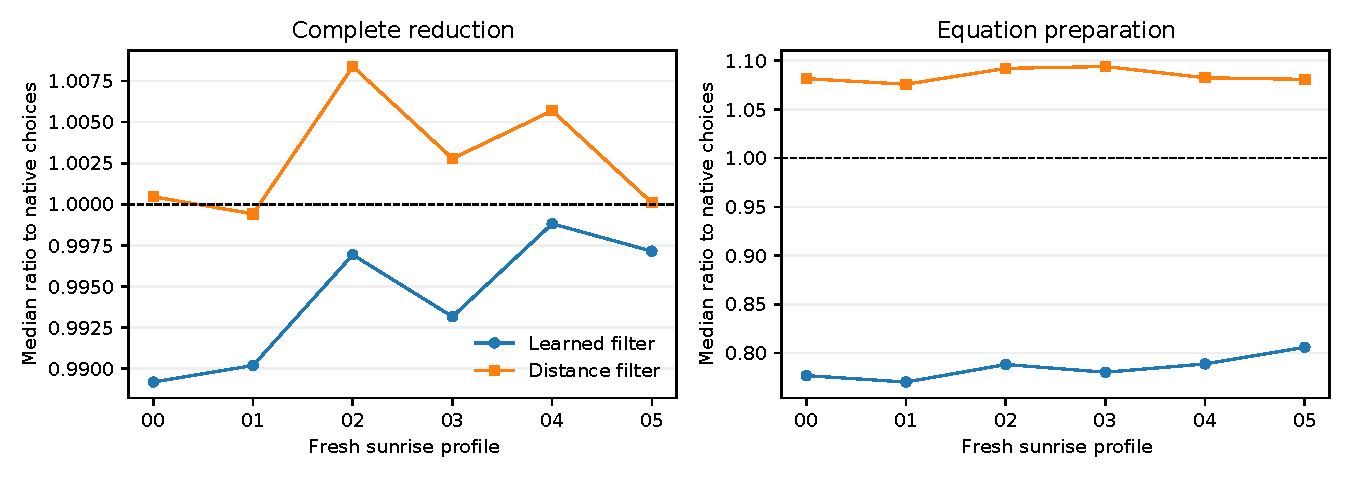
\includegraphics[width=\textwidth]{figures/equation_confirmed_costs.pdf}
 \caption{Fresh confirmation of the restricted sunrise deployment.
 Each profile uses nine repetitions for each method. Complete and
 preparation times include prediction and fallback costs.}
 \label{fig:equation-confirmed}
\end{figure}
The application interface enables this equation policy when it runs with native seed and row choices. Requests for either earlier learned policy retain native equation choices. This guard avoids the slower measured three-model combination.
The broader initial route and its slower vacuum results remain available
as experimental evidence. The measured domain contains two-loop sunrise
integrals with the stated target set, and extension to other target sets
or topologies requires further independent evidence~\cite{KiraEquationSelectionData}.
\FloatBarrier

\clearpage
\subsection{Predicting equations before constructing their coefficients}
\label{sec:early-equation-selection}
The preceding equation model first inspects a constructed identity, so its
initial prediction still requires that identity's coefficients. To reduce
this cost, we train a new version of the same model that uses only the seed,
the operator and the requested targets. This moves the decision to the point
where Kira can avoid constructing an omitted identity.

A diagnostic study motivates this change. In twelve exact native runs,
equation preparation forms the largest recorded block in the 128-target
three-loop ladder reductions. The two ladder profiles have median
preparation intervals of 1.41 and 1.23 seconds, within complete times of
4.23 and 4.36 seconds. Initial family preparation and equation preparation
together account for about 54--55\% of those times. These diagnostic
intervals come from logged stage boundaries and include wrapper costs;
the final comparison below uses the internal timers defined for this study.

For the identity in Eq.~\eqref{eq:equation-selection-identity}, the new
decision has the form
\begin{equation}
 \widehat p_{\boldsymbol\sigma,o}
 =f_\theta\!\left(\phi(\boldsymbol\sigma,o,\mathcal T)\right),
 \qquad
 \widehat p_{\boldsymbol\sigma,o}\geq\tau
 \ \Longrightarrow\ E_{\boldsymbol\sigma,o}\ \hbox{is constructed}.
 \label{eq:early-equation-decision}
\end{equation}
Here $\phi$ is the vector of features available before construction,
$f_\theta$ is the classification tree with trained parameters $\theta$,
and $\tau$ is the retention threshold. The 17 features describe the
numbers of loops, external momenta and indices, the target count, the
seed's sector, dots and numerator rank, their differences from target
limits, the distance in Eq.~\eqref{eq:equation-selection-distance},
whether the seed is itself a target, and the operator index.
The tree therefore has no need to inspect the equation's coefficients
or integral terms.

Kira supplies the ordered IBP operators, and the integration retains their
positions when it omits an equation. Several operators share the same seed
features, so we calculate those features once and store the decision for
each seed--operator pair. Kira constructs accepted equations through its
native algebra and reuses the stored decisions during later regeneration.
Symmetry identities and preferred-basis relations retain their existing
treatment. This placement reduces both repeated model work and the initial
construction of identities that the model rejects.

We retain the support-membership labels in
Eq.~\eqref{eq:equation-selection-label} and add four training batches from
two new ladder profiles. The combined collection contains 153,124 candidate
equations, including 12,270 positive labels, in fourteen batches from
eight physical profiles. These profiles contain the two-loop sunrise and
double-box and the three-loop vacuum and ladder structures. We fit trees
with maximum depths eight and twelve, using equal total weight per profile
and the same smoothed leaf frequency as before~\cite{CART1984}.
The trees contain 295 and 1,335 nodes and take 3.39 and 5.85 seconds to fit
after collection of the native training reductions. Their splits leave at least
24 and eight rows in each child, respectively. A separate implementation
check compares 918,744 decisions and finds agreement between the
stored Python features and the C++ evaluator's recomputed seed features.

The training label still describes membership in a recorded native equation
selection. It supplies neither a smallest sufficient equation set nor a
calibrated completeness probability. Kira therefore checks whether the
result expresses each target in the prescribed master basis. If the
filtered equations are insufficient, the application retries native
equations and then a larger native seed region. Exact algebra determines
all coefficients, and the benchmark additionally compares them with an
independent native reduction.

\subsection{Selecting the complete calculation on validation profiles}
We compare both trees at thresholds 0.001, 0.003 and 0.01 with native
choices and a distance filter. Repeated validation requires at least
1\% lower complete time, at least 5\% lower equation-preparation time
and no fallback before activating an early filter. We then measure
combinations with the existing seed and row models. An additional model
must lower complete time by at least 1\% relative to early filtering
alone and require no fallback in validation.

The validation record contains 77 initial candidate and control workflows,
84 repeated candidate workflows, 72 row-composition workflows and
96 seed-composition workflows. A second vacuum profile checks another
mass pattern in the composition stage. Adding the row model gives less
than 1\% incremental saving in the ladder and vacuum comparisons and
increases double-box time. Seed combinations require extra attempts for
some larger double-box and vacuum batches. These costs remain in the
comparisons and prevent those combinations from meeting the activation rule.

Validation therefore selects the depth-twelve tree for double-box batches
and the depth-eight tree for vacuum and ladder batches, with $\tau=0.01$.
The final route retains native seed and row choices. It keeps the preceding
equation policy for the recorded 21-target sunrise batch, where early
filtering fails the validation activation rule. Other structures and
ordered target lists use the preceding guarded route. This selection
minimizes measured cost among the eligible validation candidates; it does
not establish a globally fastest reduction.

We preserve an excluded preliminary collection whose proposed additional
profiles overlapped earlier reserved definitions. We replace those profiles
before the final collection and exclude every provisional row, model and
outcome from the results above. The final training, validation and test
profiles are distinct. They can share topologies, target indices and
lower-sector integral structure.

\subsection{Independent complete-reduction comparison}
We fix the models, integration, thresholds and target domains before testing
eight additional physical profiles. Two profiles belong to each of the
sunrise, double-box, vacuum and ladder structures. Sunrise uses 21 targets,
and each remaining profile uses batches of 32 and 128 targets.
Five alternating repetitions compare native choices, the preceding release,
the deployed early policy and the validation-selected distance filter.
This gives 280 complete comparison workflows. The same new binary runs
the native, early and distance arms; the preceding release uses its saved
binary and policy. The native control includes the existing project
runtime improvements and switches off learned choices.

The profiles fix rational squared masses and external invariants, while
$d$ remains symbolic. The sunrise squared masses are $(2,7,11)$ and
$(3,7,13)$, with $p^2=-101$ and $-103$, respectively.
The double-box pairs are $(s,t)=(-101,-103)$ and $(-107,-109)$.
The vacuum squared-mass vectors are $(1,1,1,1,1,11)$ and
$(1,1,1,13,13,13)$, and the ladder squared-mass vector is
$(1,0,0,0,0,0,0,0)$ with $p^2=-101$ and $-103$.
Here $p$ is the external momentum of each two-point family, and $s$ and $t$
are the independent four-point invariants of the double-box family.
These values use the common mass scale of the family definitions.
The coefficient comparisons therefore take place in $\mathbb Q(d)$,
the field of rational functions of $d$ with rational coefficients.
The graph structures and ordered target lists are known from development;
the new profiles test transfer across masses and invariants within that domain.

Complete time includes route selection, input preparation, model loading
and evaluation, Kira startup, IBP generation, exact algebra, basis and
coefficient checks, cleanup and every fallback. The comparison driver is
already running. Independent reference and master-basis preparation,
the later independent audit and compression of retained results lie outside
the timer. Equation-preparation time includes modular generation,
selection and solving, together with symbolic equation regeneration.
These internal intervals differ from the broader diagnostic intervals
used to locate the initial bottleneck.

We take the median of five repetitions within each batch, average logarithmic
time ratios over sizes within a physical profile, and give each profile
equal weight. Descriptive 95\% intervals resample whole profiles
10,000 times. For methods $A$ and $B$, the reported ratio is
\begin{equation}
 R_{A/B}=
 \exp\!\left[
 \frac{1}{G}\sum_{g=1}^{G}\frac{1}{|B_g|}
 \sum_{b\in B_g}
 \log\frac{\widetilde T_{A,b}}{\widetilde T_{B,b}}
 \right],
 \label{eq:early-cost-ratio}
\end{equation}
where $G$ is the number of physical profiles, $B_g$ is the set of batches
for profile $g$, and $\widetilde T_{A,b}$ is the median complete time for
method $A$ and batch $b$. The same expression applies to preparation time.
A ratio below one means that method $A$ uses less time.

The deployed policy has a complete-time ratio of 0.943 to native choices, with descriptive interval $[0.915,0.970]$, and a preparation ratio of 0.638, with interval $[0.546,0.734]$. These correspond to 5.7\% lower complete time and 36.2\% lower preparation time in the profile-weighted comparison. Its complete-time ratio to the preceding release is 0.943, with interval $[0.912,0.974]$. Its ratio to the distance control is 0.934, with interval $[0.904,0.965]$.

For the two-loop sunrise profiles, the complete-time ratio is 0.986 and the preparation ratio is 0.819. For the two-loop double box profiles, the complete-time ratio is 0.884 and the preparation ratio is 0.655. For the three-loop vacuum profiles, the complete-time ratio is 0.958 and the preparation ratio is 0.453. For the three-loop ladder profiles, the complete-time ratio is 0.947 and the preparation ratio is 0.681. 

Across fourteen batches, native median complete times range from 0.593 to 2.709 seconds, and deployed medians range from 0.589 to 2.579 seconds. Summing one median per batch gives 21.83 seconds for native choices and 20.28 seconds for the deployed route. This workload sum uses a different weighting from Eq.~\eqref{eq:early-cost-ratio}.

\begin{figure}[htbp]
 \centering
 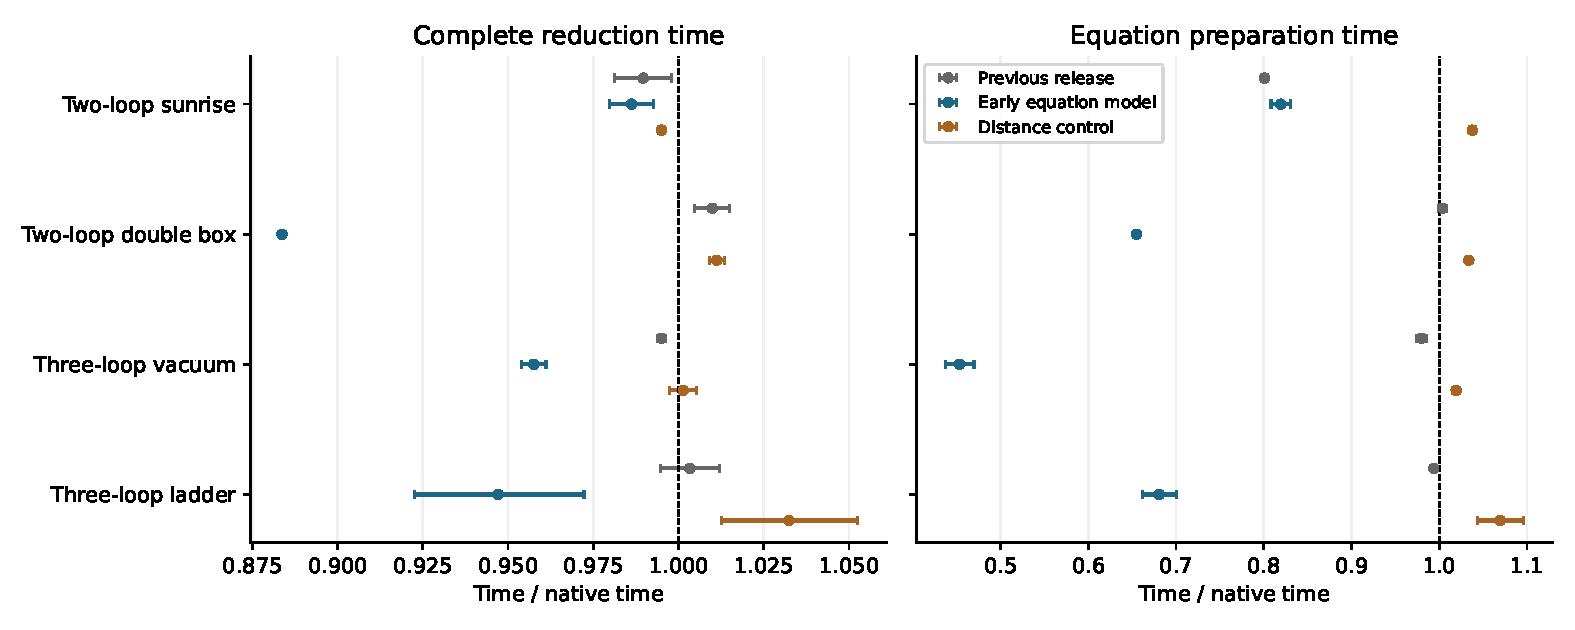
\includegraphics[width=\textwidth]{figures/early_equation_costs.pdf}
 \caption{Complete and equation-preparation time relative to native choices.
 Points use physical-profile weighting and intervals resample profiles.
 Each topology has two new physical profiles.}
 \label{fig:early-equation-costs}
\end{figure}
\begin{figure}[htbp]
 \centering
 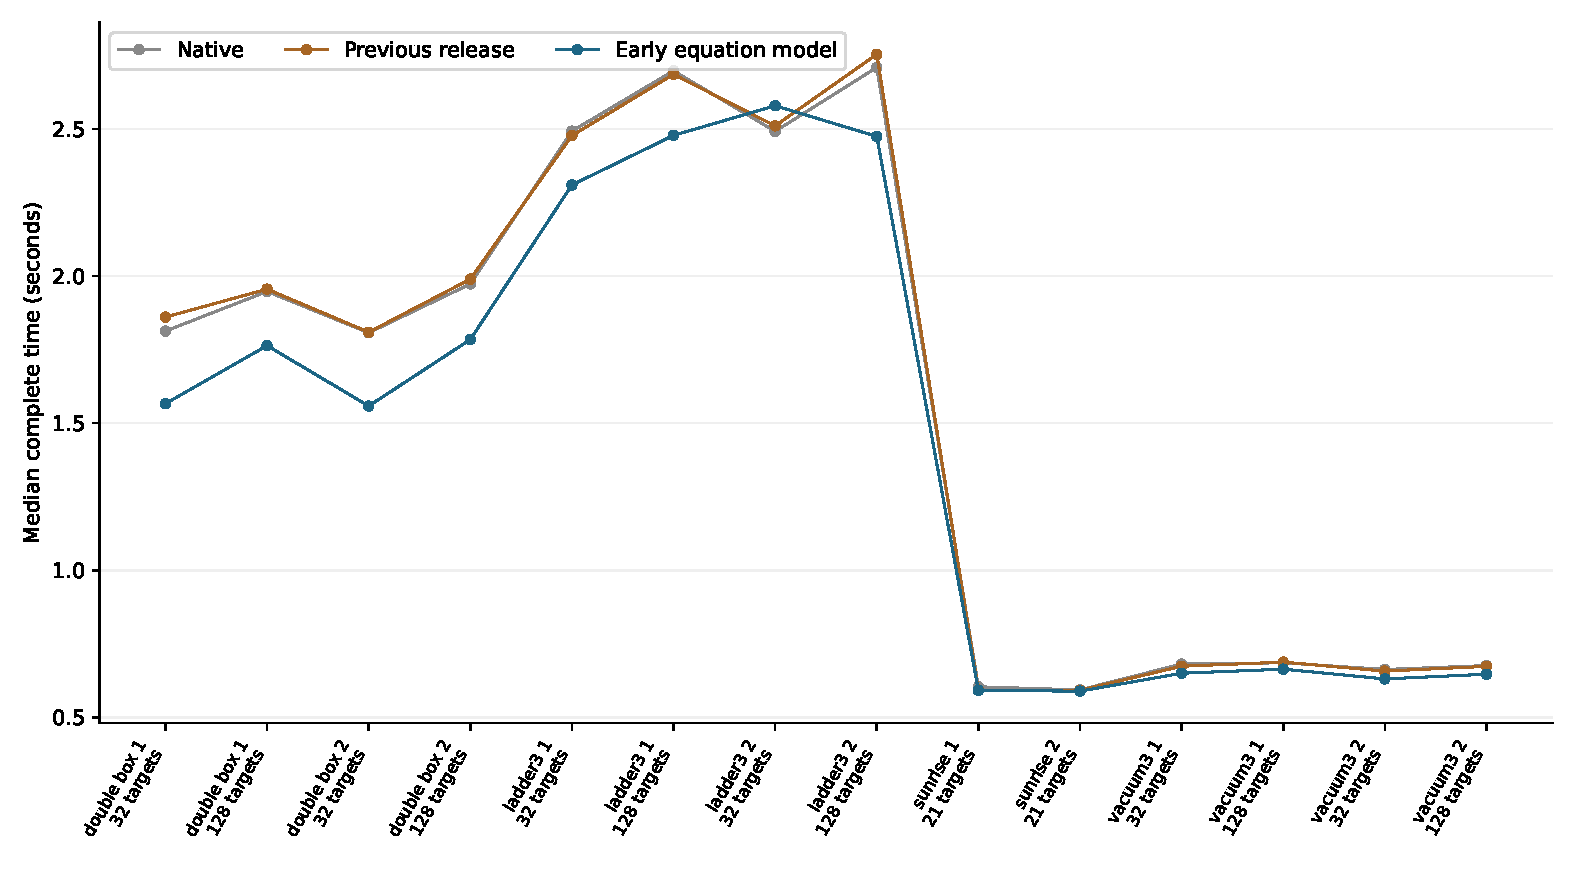
\includegraphics[width=\textwidth]{figures/early_equation_batches.pdf}
 \caption{Median complete time for each fixed target batch, including
 inference, exact checks and all fallback attempts. Each point is the
 median of five alternating repetitions.}
 \label{fig:early-equation-batches}
\end{figure}

All 280 comparison workflows and 8 additional applications pass the independent exact audit. The applications receive only the prescribed basis, and their coefficients agree with the reference after execution. The audit checks 94,970 coefficient pairs, including 1,915 distinct pairs. Every method completes on its first attempt. Maximum sampled memory for Kira and its child processes is 53.46 MiB, and maximum temporary solver storage is 1.39 MiB.

These results test a trained decision before native equation construction,
with complete costs and exact output checks. They establish the measured
domain at fixed rational kinematics. General symbolic multiscale
coefficients, new graph structures, broader target lists and high-loop
reductions require separate evidence. Section~\ref{sec:generalization} supplies subsequent tests on new scattering
structures with independent symbolic invariants. The earlier negative comparisons
remain part of the study, and the selected route activates only the
combinations supported by validation~\cite{KiraEarlyEquationData}.
\FloatBarrier

\subsection{Equation selection and shared reductions at higher loop orders}
\label{sec:higher-loop-acceleration}
The preceding native comparisons cover specific structures with two or three loops. To study the higher orders already present in the integral
collection, we now use the coupled vacuum family in
Eq.~\eqref{eq:coupled-vacuum}. This family has one power of each massless
denominator and two to four distinct massive denominators that depend on
the same momentum \(Q\). Its Euler identities and mass partial fractions
remain valid for any positive integer number of loops. This structure
allows us to test every order from one through twelve with an exact
reference, while keeping the family restriction explicit.

The dependence on the loop order suggests a further reduction in repeated
work. Let \(B=\sum_j b_j\), retain the squared-mass scale \(\mu\), and define
\begin{equation}
 z=L(d-2),\qquad
 W^{(L)}_{\boldsymbol b}=\mu^{B-1}V^{(L)}_{\boldsymbol b}.
 \label{eq:loop-shared-variable}
\end{equation}
The rescaling gives every \(W^{(L)}_{\boldsymbol b}\) the same mass dimension
as the masters \(M_j^{(L)}\). Equations~\eqref{eq:higher-loop-euler} and
\eqref{eq:higher-loop-partial-fraction} then become
\begin{align}
 0&=(z-2B)W^{(L)}_{\boldsymbol b}
       +2\sum_j b_j\rho_j W^{(L)}_{\boldsymbol b+\boldsymbol e_j},
 \label{eq:loop-shared-euler}\\
 0&=(\rho_i-\rho_j)W^{(L)}_{\boldsymbol b}
       -W^{(L)}_{\boldsymbol b-\boldsymbol e_i}
       +W^{(L)}_{\boldsymbol b-\boldsymbol e_j}.
 \label{eq:loop-shared-mass}
\end{align}
Here \(\rho_j\) is the positive squared-mass ratio defined earlier, and the
second identity requires \(b_i,b_j>0\).
The coefficient equations depend on \(L\) only through \(z\). We can
therefore solve one system over \(\mathbb Q(z)\) at fixed rational mass
ratios and obtain
\begin{equation}
 V^{(L)}_{\boldsymbol b}
 =\mu^{1-B}\sum_{j=1}^{R}
 C_{\boldsymbol b j}\bigl(L(d-2);\boldsymbol\rho\bigr)M_j^{(L)}.
 \label{eq:loop-shared-result}
\end{equation}
Each \(C_{\boldsymbol b j}\) is a polynomial in \(z\) with rational
coefficients in the present domain. The master integrals retain their
physical dependence on \(L\). The shared calculation supplies their
reduction coefficients.

We next reduce the number of identities passed to Kira. For a mixed
integral, the model scores each allowed pair \((i,j)\) in
Eq.~\eqref{eq:loop-shared-mass}. The selected identity replaces that integral
with two integrals of total massive power \(B-1\). We repeat the choice for
the resulting integrals and merge repeated dependencies across the target
batch. An integral with only one massive denominator uses
Eq.~\eqref{eq:loop-shared-euler} at the seed
\((k-1)\boldsymbol e_j\) to reduce power \(k\). At \(B=1\), the integral
belongs to the prescribed master basis. This decreasing total power
proves termination and sufficiency for every allowed model choice. Mass
partial fractions carry no IBP seed; the saved dependency choices also
determine the actual Euler seeds with one massive denominator.

The training reference counts the distinct nonmaster integrals in
recursively chosen dependency sets. If \(\mathcal D(\boldsymbol b)\)
denotes such a set, the candidate cost is
\begin{equation}
 c(\boldsymbol b;i,j)=
 \left|\{\boldsymbol b\}\cup
 \mathcal D(\boldsymbol b-\boldsymbol e_i)\cup
 \mathcal D(\boldsymbol b-\boldsymbol e_j)\right|.
 \label{eq:loop-choice-teacher}
\end{equation}
Every pair tied for the smallest candidate cost receives label one.
The recursion fixes a valid local reference and does not establish the
minimum cost for an entire target batch. We train small classification
trees using the ordered massive powers, pair positions, active-denominator
count and simple power summaries. There are 18 features, with no loop order
feature. The absence of \(L\) follows from
Eqs.~\eqref{eq:loop-shared-euler}--\eqref{eq:loop-shared-mass}.
A leaf score is an empirical training frequency. The runtime selects the
highest score and uses exact identities for the algebra. For two active
massive denominators, the single available pair is selected directly.

The training set contains 2,016 candidate actions in
546 exponent shapes, with total power through nine.
We fit depth limits four, eight and twelve using a minimum child size of
four examples. Validation selects the depth-4 candidate, which
contains 15 nodes. On 277 distinct development coefficients, the reader
agrees with symbolic algebra and takes 0.159 seconds,
compared with 4.149 seconds for the symbolic
reader. This reading improvement applies to every comparison arm and is
separate from the learned decision.


Kira solves each selected system through its interface for supplied
systems~\cite{Kira2,Kira3}. We generate the Euler and mass identities
within the measured workflow and use the same native elimination policy
for every comparison arm. This experiment measures supplied-identity
reductions. It does not measure Kira's native generation of a general
IBP system at higher loop orders. The earlier native benchmarks retain that separate
role.

The integration reads the exported coefficients with bounded rational
polynomial arithmetic and checks that polynomial division leaves zero
remainder. Development comparisons against symbolic algebra check this
reader independently. The final check uses the Taylor partial fraction
formula in Eq.~\eqref{eq:higher-loop-reference}, which does not follow the
selected dependency path. The workflow rejects unresolved nonmaster
integrals and retains a fallback to the full equation pool. Timings include input and
model loading, selection, equation construction, Kira, coefficient reading,
substitution, verification and any fallback. We also report external
process times, which include Python startup and evidence writing.
Queue waiting time and offline training are excluded.

The refined validation contains 144 workflows on six batches of mass profiles.
It compares the three trees with first-pair, smallest-pair, largest-pair and
extreme-pair rules and the full pool. Each candidate has three repetitions.
The extreme-pair rule chooses an active denominator with the smallest
power and one with the largest power. Validation selects the
extreme route; the selected learned candidate costs
1.7\% more than the selected rule.
We freeze sources, weights, profiles and target lists before 90 reserved
workflows. The reserved set has two profiles for each of
\(R=2,3,4\), with maximum powers eight and twelve, and runs every
\(L=1,\ldots,12\). Some exponent shapes with lower powers also occur in
training; the cases with maximum power twelve extend its power bound. The tests vary
mass profiles within the same topology and do not test new graph classes.
We use three repetitions and report geometric means of the six ratios of
batch medians. Descriptive intervals resample those six batches.


For each mass profile and target batch, we compare separate reductions with the full equation pool at each \(L\), separate learned reductions, a shared reduction with the full equation pool in \(z\), a shared reduction with a simple rule, and a shared learned
reduction. The full pool contains Euler seeds through the largest target
power and all mass-pair identities through one additional power. The
control with a simple rule uses the rule selected on validation. All arms use the
same project Kira binary with the earlier runtime improvements and native
row choices. These controls separate the benefit of exact loop reuse from
the benefit of selecting a smaller equation set.

For separate reductions at each loop order, learned selection gives
a complete-time ratio of 0.911 to the full pool, with
descriptive interval \([0.815,0.986]\).
With exact loop reuse in both arms, learned selection gives a ratio of
0.925 to the shared full pool, with interval
\([0.889,0.958]\).
The learned/shared ratio to the rule/shared control is
0.968, with interval
\([0.927,1.003]\).
These comparisons keep the incremental learned effect separate from
the exact reuse of coefficient equations.

The deployed shared route gives a complete-time ratio of
0.155 to separate reductions with the full equation pool, with interval
\([0.132,0.184]\).
This corresponds to 6.47 times faster execution of the
twelve-order workload under the stated timing definition.
Figures~\ref{fig:higher-loop-complete-time} and
\ref{fig:higher-loop-equations} show the batch costs and equation counts.
Validation fixes the deployed rule before these tests; we retain the
learned results as a measured alternative.

We separate calculation time from the cost of starting Python and archiving
the test evidence. Before those two outer costs, the separate learned
route has time ratio 0.943, with descriptive interval
\([0.873,0.995]\), to the full pool.
The time spent inside Kira has ratio 0.965, with interval
\([0.925,0.992]\).
Thus the calculation saves 5.7\% and Kira itself saves
3.5\% in this comparison. Archiving fewer source
equations contributes to the larger saving in external process time.

With shared coefficients, the ratio of calculation times of the learned route
to the full pool is 0.966, with interval
\([0.941,0.982]\).
Its ratio to the control with a simple rule is 0.997, with interval
\([0.984,1.011]\).
This comparison does not establish an added advantage over the simple rule.
The deployed shared calculation has ratio 0.128 to separate
calculations with the full equation pool, with interval
\([0.102,0.164]\).
The exact change of variable supplies the main reduction in repeated work.


\begin{figure}[htbp]
 \centering
 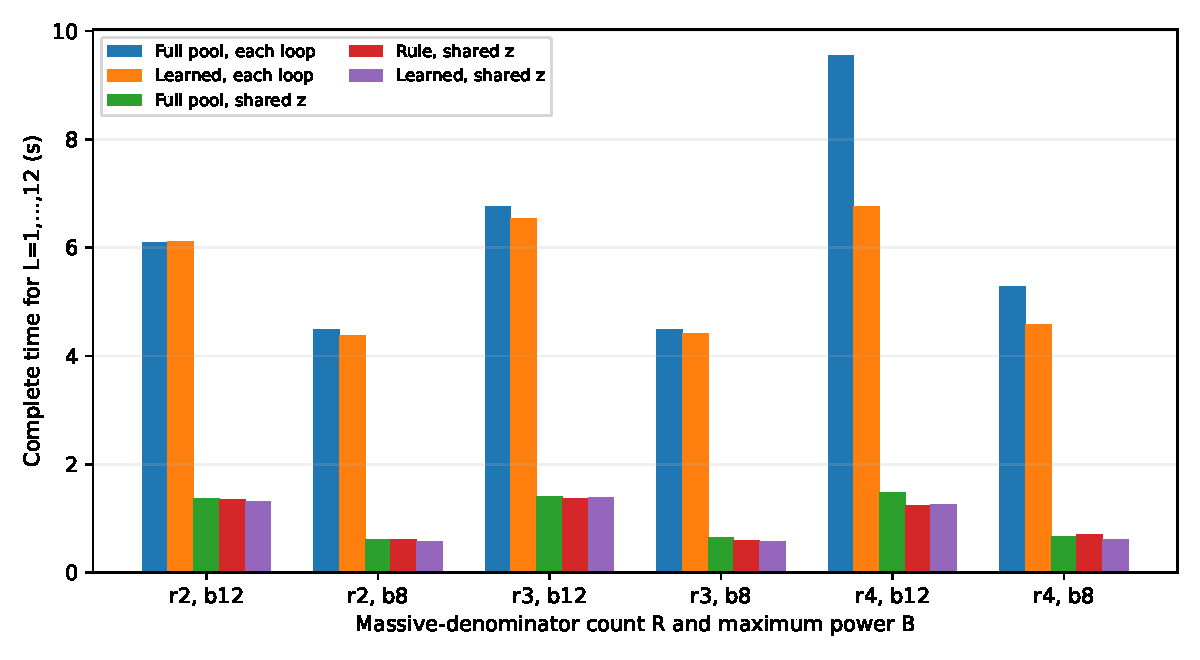
\includegraphics[width=0.98\textwidth]{figures/higher_loop_complete_times.pdf}
 \caption{Median external complete times for the twelve loop orders in
 each reserved batch. Each bar includes the full cost of its stated
 workflow. The shared methods solve once in \(z\) and check the substituted
 coefficients separately at every requested loop order.}
 \label{fig:higher-loop-complete-time}
\end{figure}

\begin{figure}[htbp]
 \centering
 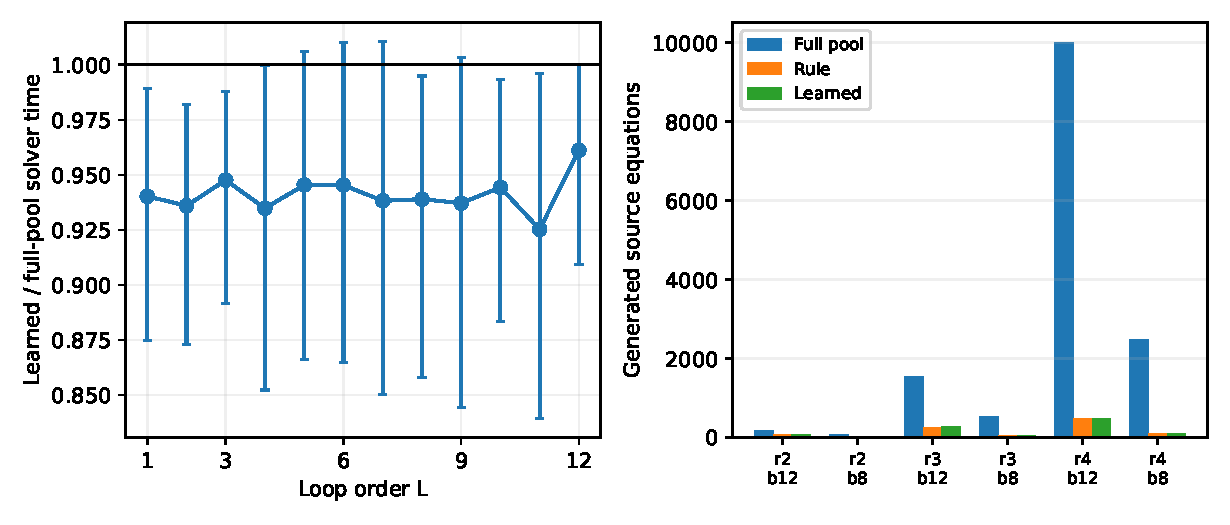
\includegraphics[width=0.98\textwidth]{figures/higher_loop_equations.pdf}
 \caption{Separate-loop solver-time ratios and generated equation counts.
 The left panel includes construction, prediction, Kira and coefficient
 reading for each loop order; the complete workflow also includes the
 checks shown in Fig.~\ref{fig:higher-loop-complete-time}. The intervals
 describe variation across the six reserved batches.}
 \label{fig:higher-loop-equations}
\end{figure}

All 90 reserved workflows and six additional applications pass exact
checks. The extra applications use loop orders 13, 16, 24 and 32.
The audit checks 65,504 coefficient positions, including
5,696 distinct positions, across
492 Kira calls. It finds 0 failed attempts
and 0 fallback workflows.
The largest sampled memory of Kira and its child processes is
23.05 MiB, and the largest temporary
solver storage is 0.58 MiB.
The analytic reference also supplies a direct reduction for this
special family. The reported comparisons measure routes that use Kira.


Equation~\eqref{eq:loop-shared-result} holds for any positive \(L\) in this
scalar family. The finite tests cover the stated orders. Generic scattering
families contain additional scalar products, numerator powers and kinematic
variables, so their native IBP reduction needs separate tests. These results
apply to the stated coupled vacuum family and supplied
identities~\cite{KiraHigherLoopData}.


\subsection{Learning equation choices for groups of targets}
\label{sec:batch-reuse}
The shared variable in Eq.~\eqref{eq:loop-shared-variable} removes repeated
reductions at different loop orders. We now reduce repeated work within
each target set and across independent mass profiles of the same restricted
vacuum family. The calculation still uses one power of every massless
denominator and \(R=2,3,4\) distinct massive denominators. Kira performs
exact elimination on the supplied Euler and partial-fraction identities,
and the retained native IBP-generation interfaces continue to serve their
previously tested two- and three-loop domains.

For a target set \(\mathcal T\), let \(\pi\) specify an ordering of the
\(R\) massive denominators. At each mixed integral, we use the first two
active denominators in this ordering in Eq.~\eqref{eq:loop-shared-mass}.
Every resulting integral has a smaller total power \(B\), and repeated
integrals share the same subsequent reduction. Let
\(\mathcal D_\pi(\mathcal T)\) be the resulting set of distinct nonmaster
integrals. To train a model that favors small shared systems, we assign
the cost
\begin{equation}
 S_\pi(\mathcal T)=
 \sum_{\boldsymbol b\in\mathcal D_\pi(\mathcal T)}
 \left(3\sum_{j=1}^{R}b_j-2\right).
 \label{eq:batch-weighted-cost}
\end{equation}
The weight increases with the number of polynomial coefficients that can
enter a substitution. It provides a training measure of algebraic work;
actual Kira operation counts and the cost of large rational numbers also
depend on its elimination and simplification choices. The smallest
\(S_\pi\) among the \(R!\) mass orderings supplies a restricted reference
for the quality of a choice. More general reduction paths can have
different costs.

We train ensembles of four and sixteen extremely randomized regression
trees~\cite{Geurts2006ExtraTrees} to predict \(\log S_\pi\), then select the
ordering with the smallest predicted value. The 32 inputs describe the
target count, number of massive denominators, total powers, the mean and mean squared power at each
position of \(\pi\), the largest power, the fraction of targets with that
denominator present, and pairwise mean minima and products of powers.
These inputs describe sharing across the entire target set. Each prediction estimates the reduction cost, while exact identities
and Kira determine the reduction coefficients. Two massive denominators admit a single pair, so those
requests bypass inference.

The training set contains 420 target batches and 6,300 candidate orderings,
with total powers up to fourteen and at most 128 targets per batch.
Both ensembles have maximum depth twelve and at least three training
examples per leaf. We compare their complete calculation times with
four simple ordering rules, the earlier learned pair selector, and
enumeration of all fixed orderings. The first validation uses 324
calculations on twelve new mass profiles and selects the four-tree
ensemble as the cheaper learned candidate. Its time ratio to the
fastest simple rule is 1.000, so single-profile deployment
retains that rule. A further 48 validation applications combine three
profiles at a time and give a learned-to-simple time ratio of
0.925, which selects learned ordering for that route.

The selected trees require 7634 nodes in total. We also store their
unchanged thresholds and leaf values in compiled inference routines to
reduce loading and prediction cost. All 12,600 compared candidate scores
agree exactly with the original tree evaluation. For the selected
ensemble, compiled evaluation takes 0.921 times the Python
decision time over the training batches. Fresh complete-calculation
validation then chooses the inference implementation used for production calculations; this comparison includes
model loading and inference and measures the time of the complete calculation.

\subsubsection{Sharing exact checks and Kira calls}
The original shared reduction still expanded and checked the same
coefficient separately at each requested loop order. We instead compare
the Kira coefficient \(C_{\boldsymbol b j}(z)\) with an independent
Taylor partial-fraction construction directly in \(\mathbb Q[z]\).
Exact equality in this polynomial ring implies equality after the
substitution \(z=L(d-2)\) for each requested \(L\). Every returned
coefficient therefore keeps an exact check while each symbolic comparison
takes place once.

We also use integer polynomial arithmetic when reading the coefficients
and applying the substitution. If
\(C(z)=D^{-1}\sum_{n=0}^{q}a_nz^n\), where the \(a_n\) are integers and
\(D\) is a positive common denominator, then the coefficient of \(d^k\)
after substitution is
\begin{equation}
 [d^k]C\bigl(L(d-2)\bigr)
 =\frac{1}{D}\sum_{n=k}^{q}a_n L^n
   \binom{n}{k}(-2)^{n-k}.
 \label{eq:batch-integer-substitution}
\end{equation}
Here \(q\) is the polynomial degree and \([d^k]\) denotes extraction of
the coefficient of \(d^k\). This form keeps the inner sums in integer
arithmetic and reduces the number of repeated fraction normalizations.
These savings follow from exact algebra, separately from the learned
choice of equations.

Independent mass profiles can also share a Kira invocation. We give each
profile its own integral identifiers and master basis, then form
\begin{equation}
 A=\operatorname{diag}(A_1,\ldots,A_P),\qquad
 A\begin{pmatrix}\boldsymbol I_1\\ \vdots\\ \boldsymbol I_P\end{pmatrix}
 =0.
 \label{eq:batch-independent-systems}
\end{equation}
Here \(P\) is the number of profiles, \(A_p\) is the coefficient matrix
of the selected identities for profile \(p\), and \(\boldsymbol I_p\)
contains its integrals. Kira reduces this combined system in one call.
The output checks require each target to contain only masters of its own
profile, after which the same independent symbolic checks apply.
The learned model chooses the equations for each profile before assembly.
The current interface admits up to eight profiles, 512 targets and
12,000 selected equations per call. The timing tests use three profiles
per call. A failed combined reduction retries the profiles separately,
and a failed selected system uses the preserved full supplied system.

\subsubsection{Independent timing and correctness results}
The first reserved comparison uses twelve new mass profiles, powers up to
fourteen, up to 96 requested targets per profile and every loop order
from one through twelve. Five repetitions of five methods give 300
complete calculations. The learned route with shared checks has time
ratio 0.394 to the preceding release, with descriptive interval
\([0.314,0.487]\). Its ratio to the updated simple rule is 0.986,
with interval \([0.955,1.019]\). These measurements separate the common
arithmetic improvements from the additional equation-choice model.
The mean weighted-cost ratio to the best enumerated mass ordering is
1.035. This reference concerns Eq.~\eqref{eq:batch-weighted-cost}
within the finite set of mass orderings.

We then compare separate and combined reductions on four groups of
three of these profiles. Eighty complete applications give a
combined-to-separate learned time ratio of 0.516, with interval
\([0.485,0.563]\). Within combined calculations, the learned-to-simple ratio
is 1.025, with interval \([0.941,1.121]\). This comparison counts
the model cost on both sides where the model is used.

A second reserved set contains twelve further mass profiles, powers up
to thirteen and up to 80 requested targets per profile. Eighty
applications compare the preceding separate workflow, the updated
combined simple rule, and both learned inference implementations on the same
four groups. The compiled learned route has complete-time ratio
0.218 to the preceding workflow, with interval \([0.169,0.276]\), and
ratio 0.923 to the combined simple rule, with interval
\([0.885,0.962]\). Its ratio to Python inference in the otherwise
identical learned workflow is 0.990, with interval
\([0.885,1.117]\). The two learned implementations produce identical selected
equation systems. Complete-time validation retains the Python learned inference implementation for combined requests and the simple rule for a single profile. The compiled inference implementation remains available with its measured comparison.

All 460 reserved applications pass exact checks without fallback.
Separate integration checks cover loop orders 1, 12, 16, 24 and 32 and
include one deliberately failed check that successfully invokes the full
system fallback. The independent audits check 54,594 saved
coefficient occurrences in expanded loop-dependent expressions, and the
final audit also compares 21,675 raw Kira coefficient occurrences
with the earlier rational-expression reader. The peak sampled Kira
process-tree memory is 21.27 MiB and peak native scratch use is
0.75 MiB in these tests.

Complete calculation time includes input reading, model loading,
equation selection and construction, Kira execution, exact coefficient
reading, loop substitution, verification and any fallback. Separate
external-process measurements also include Python startup and evidence
archiving. Reported ratios are geometric means of batch median ratios;
the descriptive 95\% intervals resample the twelve single batches or
four combined groups. The small number of groups limits conclusions
about other workloads. Figure~\ref{fig:batch-reuse-single} shows the
single-profile comparison, and Fig.~\ref{fig:batch-reuse-packed} shows
the second combined comparison~\cite{KiraBatchReuseData}.

These results support acceleration within the stated vacuum family and
fixed mass profiles. The Taylor construction also supplies a direct
analytic solution for this family; these comparisons concern the
reductions performed through Kira here. General scattering families,
native generation of high-loop IBP systems and a globally fastest
reduction remain outside the evidence.

\begin{figure}[htbp]
 \centering
 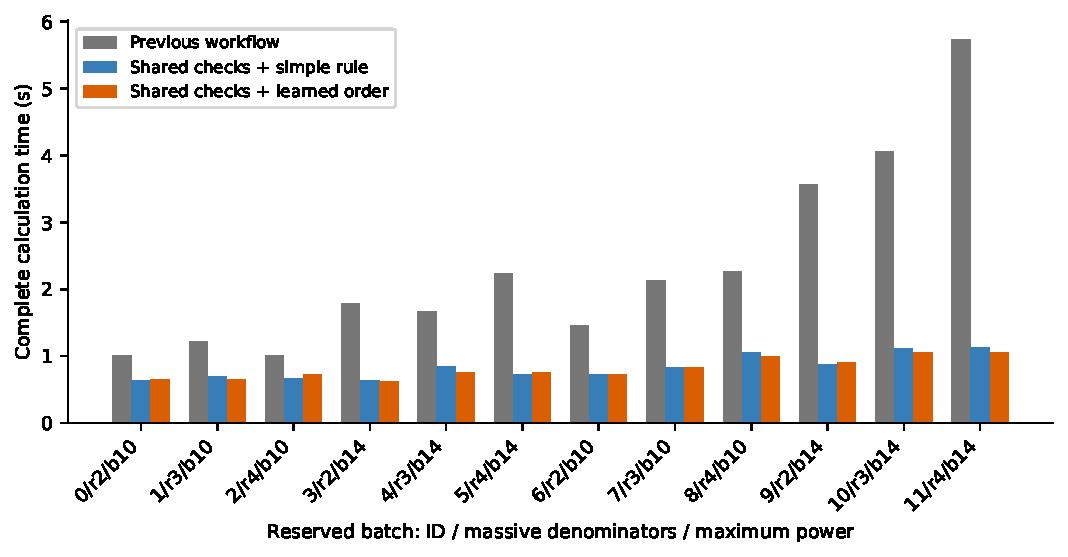
\includegraphics[width=\textwidth]{figures/batch_reuse_single.pdf}
 \caption{Median complete calculation time for the twelve reserved
 single-profile batches. All methods return the same exact reductions
 at loop orders one through twelve. The updated simple and learned
 routes share the improved exact checks and coefficient arithmetic.}
 \label{fig:batch-reuse-single}
\end{figure}
\begin{figure}[htbp]
 \centering
 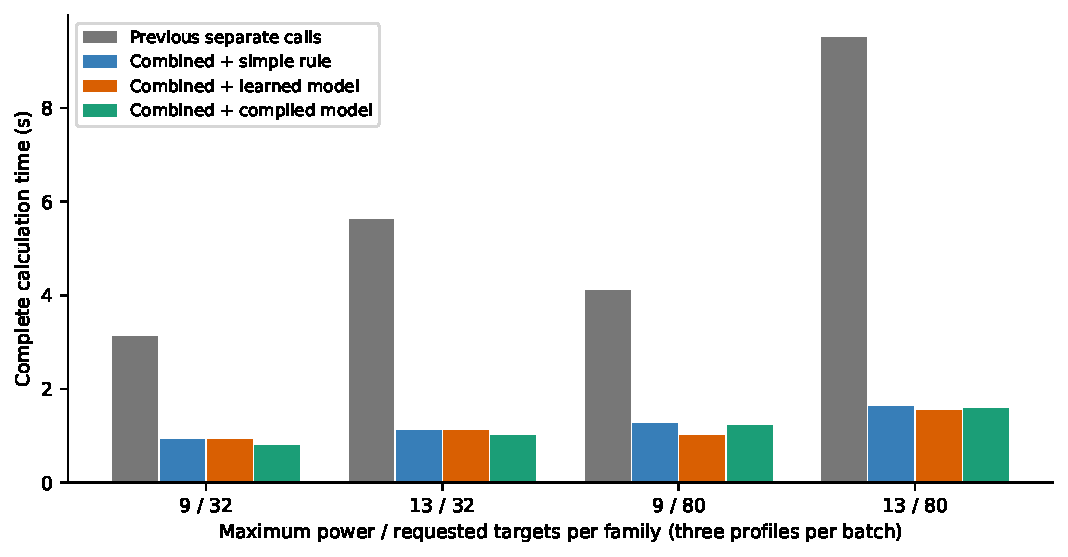
\includegraphics[width=\textwidth]{figures/batch_reuse_packed.pdf}
 \caption{Median complete time for the second reserved comparison.
 Each group contains three independent mass profiles. The previous
 route makes separate Kira calls; the other routes combine the selected
 systems. The target count on the axis is the requested count per
 profile and is capped by the available index vectors.}
 \label{fig:batch-reuse-packed}
\end{figure}


\subsection{Exact pre-reduction and a checked direct path}
\label{sec:pre-reduction}
The combined workflow in Section~\ref{sec:batch-reuse} still spends much
of its time in Kira after the model selects sufficient identities.
For the restricted vacuum family, every selected identity lowers the total
massive-denominator power. We can therefore evaluate the substitutions
in increasing order of that power and return the completed result after
an independent exact check. Kira remains available for comparison and
as a fallback when this direct path fails its checks.

Let \(\boldsymbol C_{\boldsymbol b}(z)\) be the vector of coefficients
of the prescribed masters in \(W_{\boldsymbol b}^{(L)}\), with
\(z=L(d-2)\) as defined earlier. For the master with index
\(\boldsymbol e_j\), this vector is the unit vector
\(\boldsymbol C_{\boldsymbol e_j}=\boldsymbol e_j\).
The selected mass identity gives
\begin{equation}
 \boldsymbol C_{\boldsymbol b}(z)=
 \frac{\boldsymbol C_{\boldsymbol b-\boldsymbol e_i}(z)
       -\boldsymbol C_{\boldsymbol b-\boldsymbol e_j}(z)}
      {\rho_i-\rho_j},
 \qquad b_i,b_j>0.
 \label{eq:pre-mass}
\end{equation}
Here \(\rho_i\) and \(\rho_j\) are the distinct positive mass ratios
specified for the family. When only denominator \(j\) is present,
the Euler identity gives
\begin{equation}
 \boldsymbol C_{k\boldsymbol e_j}(z)
 =\frac{2(k-1)-z}{2(k-1)\rho_j}
   \boldsymbol C_{(k-1)\boldsymbol e_j}(z),
 \qquad k\geq 2.
 \label{eq:pre-euler}
\end{equation}
Both formulas reduce \(B=\sum_j b_j\), so they terminate at the
specified masters. We evaluate each distinct intermediate integral once.

The existing four-tree model selects the mass ordering before these
substitutions, with unchanged weights and training examples.
The learned direct route uses the previously checked compiled evaluator.
We store each polynomial coefficient as integers over a positive common
denominator and cancel their common divisor after each addition or scaling. This keeps the arithmetic exact and reduces
repeated fraction normalization. The model selects the intermediate
integrals that we visit, while Eqs.~\eqref{eq:pre-mass} and
\eqref{eq:pre-euler} determine their coefficients.

An independent Taylor partial-fraction construction checks the result.
For an auxiliary dimensionless variable \(x\), define
\begin{equation}
 \prod_{i:b_i>0}(x+\rho_i)^{-b_i}
 =\sum_{j:b_j>0}\sum_{k=1}^{b_j}\frac{a_{jk}}{(x+\rho_j)^k},
 \qquad
 a_{jk}=[t^{\,b_j-k}]
       \prod_{\substack{i\ne j\\b_i>0}}
       (\rho_i-\rho_j+t)^{-b_i}.
 \label{eq:pre-taylor}
\end{equation}
Here \([t^n]\) means the coefficient of \(t^n\) in the Taylor series.
The corresponding master coefficient is
\begin{equation}
 C_{\boldsymbol b j}(z)=
 \sum_{k=1}^{b_j}a_{jk}
 \prod_{h=1}^{k-1}\frac{2h-z}{2h\rho_j}.
 \label{eq:pre-independent}
\end{equation}
An empty product equals one. This construction uses the same exact
single-denominator relation and obtains the mixed-denominator
coefficients independently of the selected pairs.
We require equality of every polynomial coefficient before substituting
\(z=L(d-2)\). A failed check retries the original request through the
preceding Kira route and its existing full-system fallback.

We compare five routes on identical targets. The preceding deployed route
sends model-selected equations to Kira. A second route first evaluates
the recurrence, then sends the completed target-to-master relations to
Kira. Three direct routes return checked coefficients: one uses learned
ordering, one uses simple extreme-power ordering, and one constructs
the answer with Eq.~\eqref{eq:pre-independent} and checks it with the
simple recurrence. The last route supplies an analytic control that
includes an independent exact check.

Six new three-profile batches provide 90 validation calculations.
Their mass ratios lie outside the ranges used in earlier training and
tests. Validation selects the simple direct route before evaluating eight
further three-profile batches with masses in a separate range.
Each profile has two, three or four massive denominators, the largest
total power is fourteen, and every request includes loop orders one
through twelve. Five repetitions of five routes give 200 reserved
calculations, all of which pass exact checks without fallback.
The independent audit checks 30924 expanded master-coefficient
positions and compares 25770 raw Kira coefficient expressions with the
earlier rational reader. Five further applications include loop orders
1, 12, 16, 24 and 32 and a deliberately failed direct check that recovers
through Kira.

The selected route has calculation-time ratio 0.306 to the preceding
combined learned workflow, with descriptive interval \([0.246,0.373]\).
Its full worker-time ratio is 0.430, with interval \([0.414,0.446]\).
Calculation time includes request reading, model loading and inference
where used, preparation, exact algebra, checks, loop substitution and
fallback. Full worker time also includes interpreter startup and saving
the output. We take the median of five repetitions per batch and then
the geometric mean of the eight batch ratios. The intervals resample
those eight batches and describe this finite comparison.

The learned direct route has calculation-time ratio 0.982
to the simple direct route, with interval \([0.971,0.997]\), and ratio
0.991 to the analytic control, with interval \([0.973,1.013]\).
The comparison does not establish a further complete-time advantage from learned ordering over both direct controls.
Pre-reduction followed by Kira has time ratio 0.927 to the
preceding route. Figure~\ref{fig:pre-reduction-times} shows the batch times.
The principal saving in the direct routes comes from finishing the exact
triangular recurrence before a Kira invocation is needed.
These measurements cover an outer reduction path for the stated vacuum
family. Native IBP-generation policies retain their previously tested
domains, and general high-loop families require separate comparisons.
The implementation, fixed choices, raw outputs and checks accompany the
measurements~\cite{KiraPreReductionData}.

\begin{figure}[htbp]
 \centering
 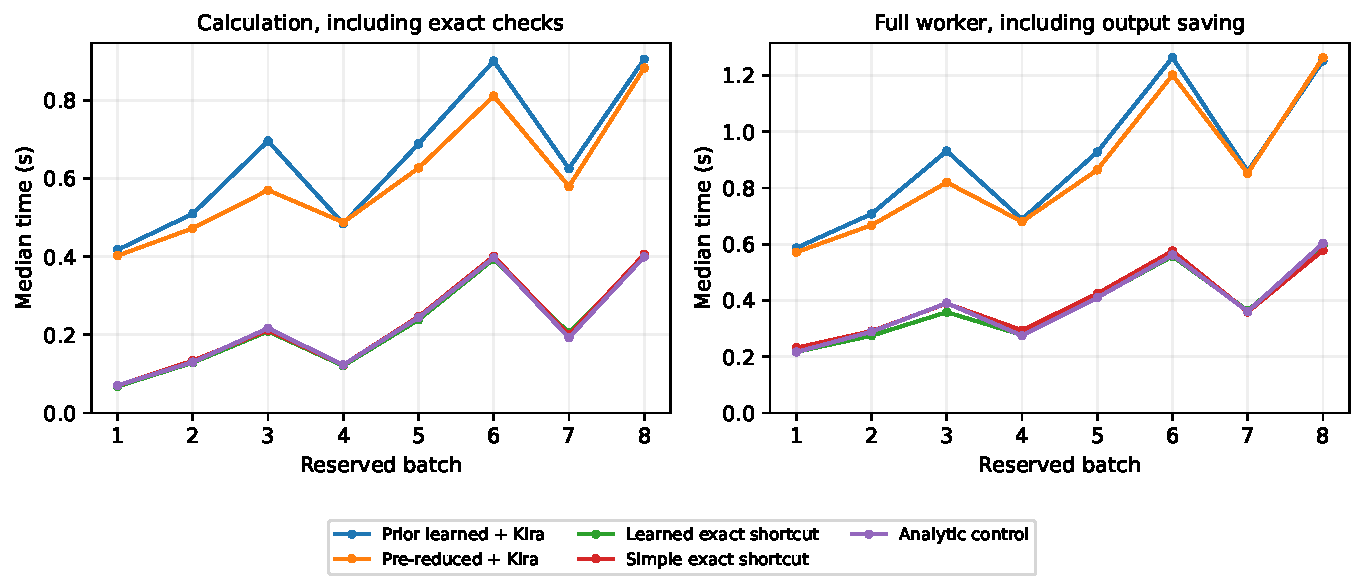
\includegraphics[width=\linewidth]{figures/pre_reduction_times.pdf}
 \caption{Reserved batch times for the preceding Kira route,
 pre-reduction followed by Kira, and three independently checked direct
 routes. Each point is the median of five complete calculations.
 The right panel includes startup and saving the output.}
 \label{fig:pre-reduction-times}
\end{figure}


\subsection{Sharing exact polynomial work across targets and loop orders}
\label{sec:polynomial-reuse}
The direct reduction in Section~\ref{sec:pre-reduction} removes the Kira
call when exact recurrence relations complete the requested reduction.
Its remaining cost includes construction of the independent check and
expansion of each coefficient at every requested loop order. We now reuse
the algebraic terms that these operations have in common and keep the
calculation process available for a bounded sequence of requests.
The master basis, selected identities and exact checks remain the same.

Write a coefficient as
\(C(z)=D^{-1}\sum_{n=0}^{q}a_nz^n\), where \(D\) is a positive integer,
the \(a_n\) are integers, and \(q\) is its degree. For each loop order
\(L\), define the integer transformation
\begin{equation}
 \begin{aligned}
 T^{(L)}_{kn}&=
 \begin{cases}
 \displaystyle\binom{n}{k}L^n(-2)^{n-k},& n\geq k,\\
 0,& n<k.
 \end{cases}
 \\[4pt]
 C\bigl(L(d-2)\bigr)&=\frac{1}{D}
 \sum_{k=0}^{q}\left(\sum_{n=k}^{q}T^{(L)}_{kn}a_n\right)d^k.
 \end{aligned}
 \label{eq:reuse-transform}
\end{equation}
Here \(k\) is the power of \(d\) and \(n\) is the original power of \(z\).
We form this transformation once for each requested \(L\) and reuse it
for all target coefficients. The present power limit gives \(q\leq13\).
We also obtain the common denominator once per symbolic coefficient,
then apply the integer transformations and cancel common factors.
This removes repeated binomial coefficients, powers and denominator
construction while retaining the full expanded result.

The independent check in Eq.~\eqref{eq:pre-taylor} contains repeated
Taylor terms. For a positive denominator power \(\beta\), a nonnegative
series index \(n\), and a nonzero mass difference
\(\Delta=\rho_i-\rho_j\), these terms are
\begin{equation}
 [t^n](\Delta+t)^{-\beta}
 =(-1)^n\binom{\beta+n-1}{n}\Delta^{-(\beta+n)}.
 \label{eq:reuse-taylor}
\end{equation}
We retain each required truncated factor within its mass profile and
multiply the factors with integer polynomials over common denominators.
We also form each single-denominator polynomial
\(\prod_{h=1}^{k-1}(2h-z)/(2h\rho_j)\) once for that profile and reuse it
in Eq.~\eqref{eq:pre-independent}. Every target still receives its own
independent master expansion and exact comparison with the selected
recurrence. This reuse changes the arithmetic work needed to construct
the check.

For a sequence of requests, one running process retains the transformation
matrices and, when requested, the unchanged trained model.
Each new mass profile receives fresh mass-dependent Taylor terms, so
a repeated integral identifier cannot transfer coefficients between
different physical inputs. The current interface bounds the retained
transforms and the number of requests per process. A failed exact
comparison retries the preserved Kira route. The previous ordering
policy remains the default, and this extension introduces no new model
training.

We compare the preceding arithmetic, shared transformations alone,
shared Taylor terms alone, and both changes together.
All routes use the same output writer, which stores each exact coefficient
block once. Four new three-profile batches provide 48 validation
calculations and select both arithmetic changes before the reserved test.
Eight further batches provide 160 calculations: four variants with five
repetitions each. The tests use two, three or four massive denominators,
total massive-denominator power \(B\leq14\), up to 96 requested targets
per profile, and every
loop order from one through twelve. Validation and reserved mass ranges
are disjoint from each other and from earlier training and comparisons.

The two changes together have calculation-time ratio 0.372 to the
preceding arithmetic, with descriptive 95\% interval \([0.343,0.402]\).
The ratio including process startup and output saving is 0.682,
with interval \([0.592,0.797]\). Shared transformations alone have
calculation-time ratio 0.701, and shared Taylor terms alone have
ratio 0.693. The combined route reduces expansion time to
0.414 of its previous value and construction time for the
independent check to 0.158.
These ratios compare batch medians and then take the geometric mean over
eight batches. The descriptive intervals resample those eight batches.
Figure~\ref{fig:polynomial-reuse-times} separates the component changes.

We then compare separate processes with one persistent process for streams
of four, four and eight batches. The eight-batch stream contains the
inputs from both four-batch streams. Three repetitions of four
configurations give 36 stream runs and 192 additional batch calculations.
All stream times include initial process startup, input reading,
calculation, exact checks and output saving.
With the updated arithmetic, process reuse has time ratio 0.524
to separate updated processes. Combining arithmetic and process reuse
has ratio 0.365 to separate processes with the preceding arithmetic.
The three specified streams overlap, so we report these descriptive
ratios without a statistical interval.
Figure~\ref{fig:polynomial-reuse-streams} gives the individual stream times.

All 352 reserved batch calculations return identical exact coefficients
across the applicable routes. The independent audit checks 28860
expanded coefficient positions with the older formula at each loop order.
Additional interface checks cover changed masses and loop orders under
the same integral identifier, continued operation after an invalid request,
the request limit, retained model evaluation, and recovery through Kira
after a deliberately failed check. These savings come from shared exact
arithmetic and reduced process startup. They apply to the restricted
vacuum family and its existing reduction interface; the earlier native
IBP-generation scope remains unchanged. The frozen implementation,
measurements and checks are available with the data~\cite{KiraPolynomialReuseData}.

\begin{figure}[htbp]
 \centering
 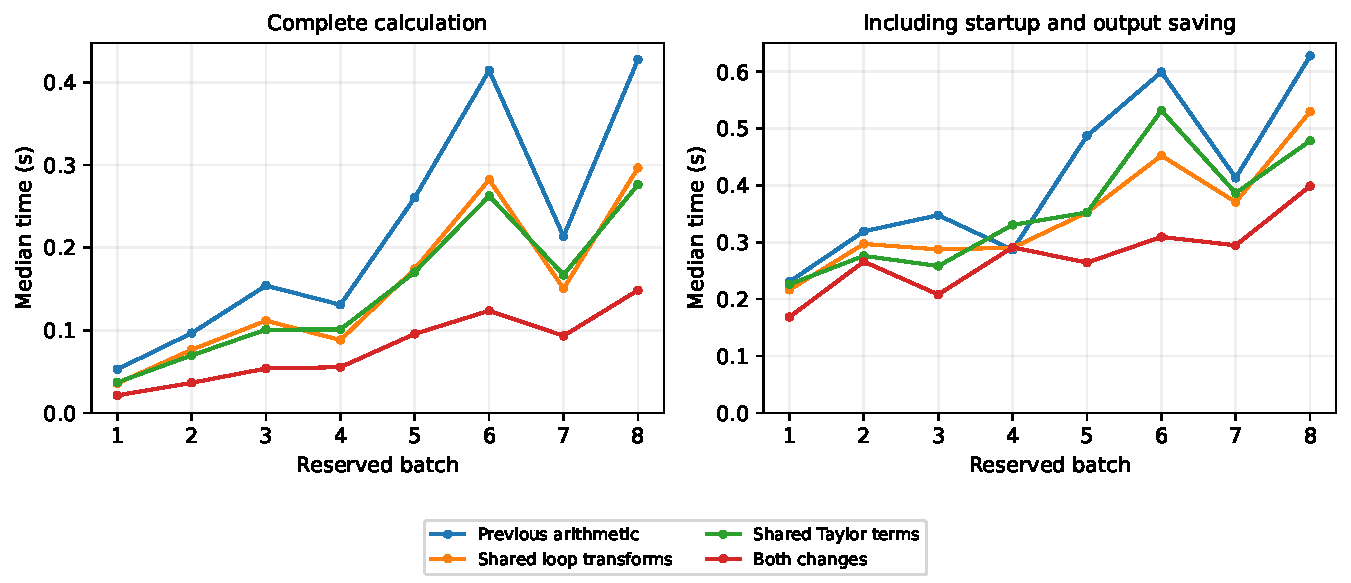
\includegraphics[width=\linewidth]{figures/polynomial_reuse_times.pdf}
 \caption{Reserved batch medians for the preceding arithmetic, each
 reuse change separately, and both changes together. Each point uses
 five complete calculations with identical target outputs and checks.}
 \label{fig:polynomial-reuse-times}
\end{figure}
\begin{figure}[htbp]
 \centering
 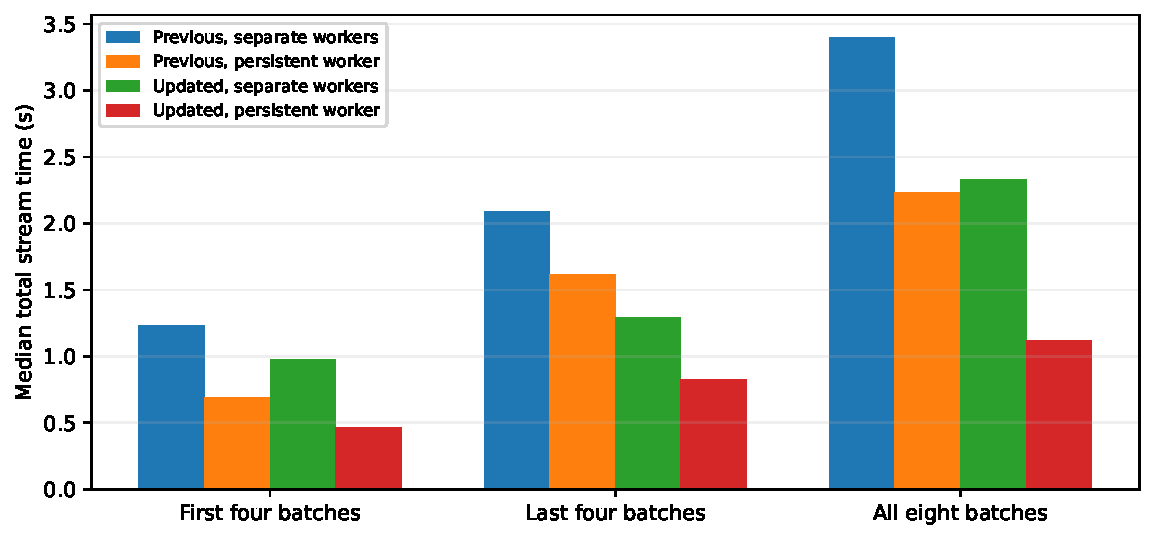
\includegraphics[width=\linewidth]{figures/polynomial_reuse_streams.pdf}
 \caption{Total time for the specified request streams, including startup,
 all exact checks and saving the results. Each bar gives the median of
 three runs. The eight-batch stream uses all inputs from the two
 four-batch streams.}
 \label{fig:polynomial-reuse-streams}
\end{figure}


\clearpage
\subsection{Exact integer arithmetic and learned batch strategies}
\label{sec:exact-backend}
Section~\ref{sec:polynomial-reuse} reuses the transformations for
\(z=L(d-2)\), but its implementation still converts coefficients between
integer polynomials and separate rational numbers. It also writes each
integer as decimal text. We now retain the common-denominator representation,
compile the loop-order expansion, and test a compact exact output format.
We then train a small model to choose a recurrence strategy for a whole
target batch and compare its cost with fixed strategies.

For a polynomial \(C(z)=D^{-1}\sum_{n=0}^{q}u_nz^n\), we store the integer
vector \((u_0,\ldots,u_q)\) and positive denominator \(D\), with
\(\gcd(D,u_0,\ldots,u_q)=1\). Both the selected recurrence and the independent
Taylor construction return this form, so their exact comparison needs
no conversion to separate fractions. The compiled expansion uses
Eq.~\eqref{eq:reuse-transform} to obtain
\begin{equation}
 v_k=\sum_{n=k}^{q}T^{(L)}_{kn}u_n,\qquad
 g_k=\gcd(|v_k|,D),\qquad
 [d^k]C\bigl(L(d-2)\bigr)=\frac{v_k/g_k}{D/g_k}.
 \label{eq:backend-integer}
\end{equation}
Here \(v_k\) is the integer numerator before cancellation, \(g_k\) is its
greatest common divisor with \(D\), and \([d^k]\) extracts the coefficient
of \(d^k\). The implementation uses integer operations from the GNU Multiple Precision
Arithmetic Library (GMP); the installed
library version is 6.0.0~\cite{GMPIntegerManual}. Every coefficient
retains its exact reduced numerator and denominator.

The compact format records the sign, byte length and base-256 digits of
each integer, together with the target, master and loop-order indices.
It therefore preserves the full symbolic and expanded coefficients.
A supplied reader recovers the same coefficient arrays as the decimal
format. We measure the cost of reading these arrays as well as the
cost of producing and saving them, so the comparison includes the
conversion needed by a consumer of the result. The same master basis,
independent Taylor check and Kira fallback apply throughout.

The learned strategy selects one of five rules for each batch.
The first rule is the preceding extreme-power rule. Two further rules
order denominator slots by their total powers across the targets,
in increasing or decreasing order. Another rule selects the active
mass pair with the largest absolute mass difference, and the last
uses a fixed slot order. Each rule generates a terminating set of
exact recurrence relations. The model can change which intermediate
integrals occur and the sizes of the rational coefficients during
substitution.

For batch \(\mathcal B\) and rule \(s\), let \(T_{\mathcal B s r}\) be the
measured time in repetition \(r\) of an already running worker.
This time includes request reading, recurrence selection, exact
arithmetic, the independent check and output writing. The training
target and the rule selected by the model are
\begin{equation}
 y_{\mathcal B s}=
 \log\!\left(\operatorname{median}_{r=1,2,3}T_{\mathcal B s r}\right),
 \qquad
 \widehat s(\mathcal B)=
 \mathop{\operatorname{arg\,min}}_s f_s(x_{\mathcal B}),
 \label{eq:backend-policy}
\end{equation}
where \(x_{\mathcal B}\) contains 49 input features and \(f_s\)
is the tree prediction of the log time for rule \(s\).
The features describe target powers, numbers of active denominators,
loop orders, masses, mass differences, and shared integrals obtained by
lowering one positive target power. We combine profile means and maxima
into a fixed-length batch description. A multi-output regression tree
with maximum depth four and at least six training batches per leaf learns
these costs; the fitted tree has 19 nodes.
The scores estimate runtime and carry no calibrated probability claim.

Training uses 96 batches and 1,440 timed calculations. The first twelve validation
batches provide 324 calculations that compare the preceding
arithmetic, retained integer polynomials, compiled expansion with decimal
output, compiled expansion with binary output, and the learned rule.
The validation also compares every fixed recurrence rule with the compiled
binary route. Each batch contains three profiles with two, three and four
massive denominators. Total massive powers reach fourteen, requested
target counts reach 96 per profile, and every profile includes loop orders
one through twelve. The training, validation and reserved test stages
use distinct targets and mass profiles.

The first validation selects retained integer polynomials with decimal
output. Its reserved comparison contains 504 batch calculations and
passes every exact check. Its full-time ratio, including output reading,
is 0.998 with descriptive interval \([0.867,1.162]\), so this comparison
does not establish a complete-time improvement. The binary variants
reduce production time, but their Python reader adds enough cost to
remove the gain in the full comparison.

We therefore compile the expanded-coefficient reader while retaining the
same binary format, exact arithmetic and trained tree. This change follows
the reader cost observed during validation. The original frozen comparison
remains intact. The compiled reader passes 1,000 loop-output comparisons
with the Python reader and rejects 250 truncated records. A new set of
twelve validation batches supplies 324 further calculations, and a separate
set of twelve test batches supplies the final reserved comparison.
An incomplete reader comparison is excluded because its selection step
referenced the earlier validation set. We preserve those 360 measurements,
correct the stage references, and freeze the prescribed choice from the
new validation set before generating results for fresh reserved targets.

The second validation selects compiled expansion and binary output with a fixed recurrence rule using total process time plus
output reading. A learned route must improve on the best fixed route by at least
two percent to replace it. We freeze the implementation, tree, deployment
choice and test inputs before the reserved comparison.
Twelve new batches then provide 300 separate-process calculations,
with five repetitions per method. The implementation comparison uses
the same request interface and output writer for matched routes.

The selected route has calculation-time ratio 0.522 to the preceding
arithmetic. Its full process-time ratio is 0.850, with descriptive
95\% interval \([0.785,0.909]\), and the ratio including output reading is
0.858, with interval \([0.800,0.914]\).
Retaining integer polynomials alone gives a ratio of 0.981 when
output reading is included. Compiled expansion with decimal output gives
0.933, and compiled expansion with binary output and the preceding
rule gives 0.858. These comparisons separate arithmetic changes
from the output format. The ratios use geometric means of within-batch
median ratios; the descriptive intervals resample the twelve batches.
Figure~\ref{fig:exact-backend-times} shows their measured times.

The learned route has total-time ratio 0.873 to the preceding
arithmetic and ratio 1.017 to the fixed rule selected by validation,
both including output reading. The latter interval is \([0.969,1.070]\).
This interval includes one, so the reserved comparison does not establish a further time reduction from learned choices. The deployed default uses the fixed validation choice.
The model and its measurements remain available with the fixed-rule
controls, including any extra inference cost.

We also compare persistent workers on three disjoint streams of four
reserved batches. Four recorded route labels and three repetitions give 36 stream runs
containing 144 additional batch calculations. The selected route has
stream-time ratio 0.702 to the preceding arithmetic, or
0.725 when reading every output is included.
Figure~\ref{fig:exact-backend-streams} separates these two costs.
The compiled fixed-rule and deployed labels use the same settings and
provide separately timed repetitions. These stream ratios describe the
three specified sequences.
A separate comparison of identical binary blocks gives compiled-to-Python
reader-time ratio 0.147, using five repetitions per reader and batch.

All 444 final reserved batch calculations pass exact comparisons,
and the two comparisons together contain 948 such calculations.
The independent audit checks 35472 expanded master-coefficient
positions against the older loop-dependent formula and verifies equality
between the two output formats. The compiled arithmetic also passes
3,277 earlier exact checks. Additional interface checks cover changed
physical inputs under a repeated identifier, invalid requests, the worker
request limit, truncated output, and recovery through Kira after a
deliberately failed independent check. These results apply to the
restricted coupled vacuum family. The earlier native IBP-generation
results retain their stated domains. The implementation, new tree,
frozen inputs and measurements accompany the report~\cite{KiraExactBackendData}.

\begin{figure}[htbp]
 \centering
 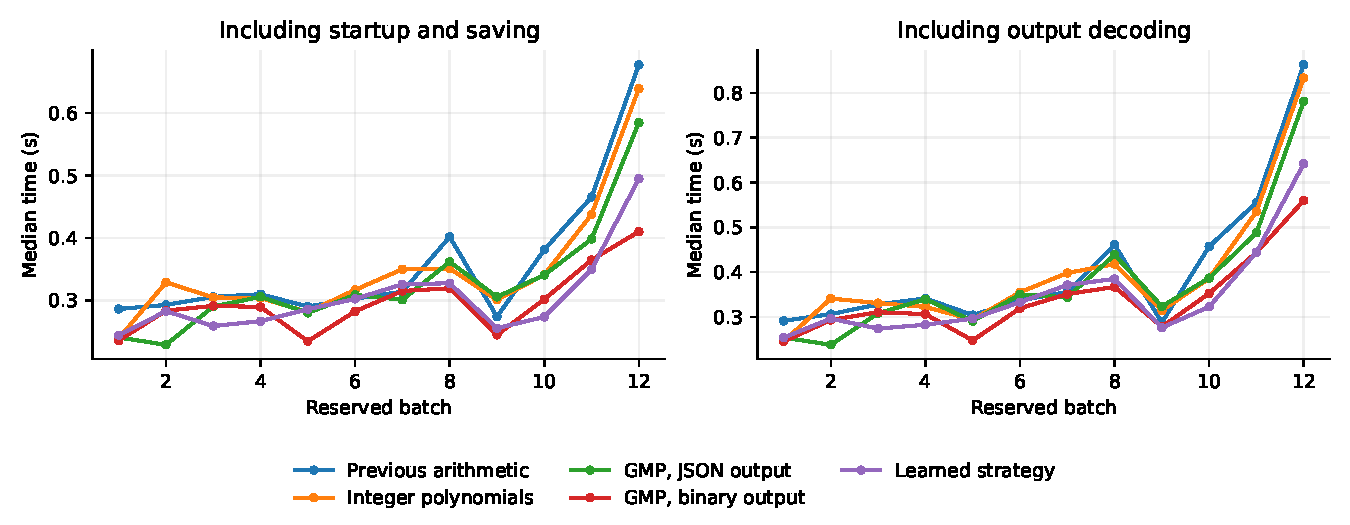
\includegraphics[width=\linewidth]{figures/exact_backend_reader_times.pdf}
 \caption{Reserved batch medians for the arithmetic and strategy variants.
 Each point uses five repetitions. The right panel includes reading and
 decoding the complete exact coefficient output.}
 \label{fig:exact-backend-times}
\end{figure}
\begin{figure}[htbp]
 \centering
 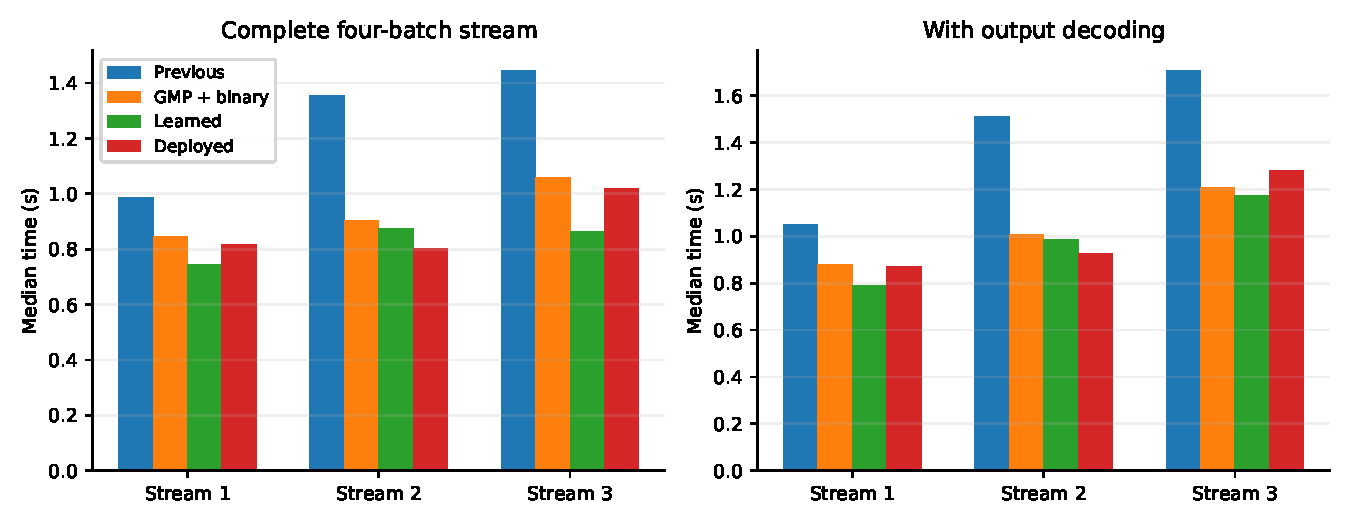
\includegraphics[width=\linewidth]{figures/exact_backend_reader_streams.pdf}
 \caption{Complete times for three disjoint four-batch streams. Each bar
 is the median of three repetitions. The right panel adds reading and
 decoding every output. The deployed route follows the validation choice.}
 \label{fig:exact-backend-streams}
\end{figure}


\clearpage
\subsection{Direct measurement of the cumulative change}
\label{sec:cumulative-speedup}
The preceding sections compare successive changes on different target sets.
To measure the cumulative change directly, we now run the original baseline
and final deployed calculation on identical integrals. We retain the
coupled vacuum family of Eq.~\eqref{eq:coupled-vacuum}, with unit massless
powers, two to four distinct massive denominators and fixed positive
integer mass ratios. We set the common squared-mass scale to \(\mu=1\),
as in the preceding comparisons. Each target has the same prescribed master basis
in every comparison.

The first control uses the saved original Kira 3.1 executable, whose file
hash agrees with the first frozen cost comparison. It generates the full
Euler and mass partial-fraction equation pool and reduces each mass
profile separately at every requested loop order. The Euler seeds extend
through the largest target power, and the mass-pair identities extend
through one additional power. A second control uses exactly the same
requests, equation generation, reader and verification, with the later
project executable used in Section~\ref{sec:higher-loop-acceleration}.
Its learned policies are disabled. Comparing these controls separates
the executable change from the subsequent removal of repeated reductions.

The final route remains the validation-selected implementation from
Section~\ref{sec:exact-backend}. It evaluates the selected recurrences directly and calls Kira only if
the exact check fails. It uses the fixed extreme-power recurrence,
shares coefficients in \(z=L(d-2)\), checks them through the independent
Taylor construction, expands them with compiled exact arithmetic and
saves lossless binary output. It retains the existing Kira fallback.
No model is retrained and no strategy is selected from the cumulative
test results. These calculations use explicitly supplied identities;
the test does not invoke native generation of a general multiloop IBP
system.

We declare eight new groups of three mass profiles, one each with
\(R=2,3,4\), and request every loop order \(L=1,\ldots,12\).
Two groups use each maximum total massive power \(8,10,12,14\).
The requested target counts per profile are \(16,32,48,64\), respectively,
capped by the available index vectors. The mass profiles are new, while
index shapes can overlap earlier data within this restricted family.
A separate upper-bound pilot checks executable compatibility and
resource use. We then freeze the implementations, executable hashes,
final deployment choice and all reserved requests.

Five repetitions of each method give 120 complete workflows.
Both controls use the same scheduler-provided job-local scratch.
Four allocated CPU slots process independent groups on one scheduled
node. Each worker binds to a distinct available physical core, and
every matched comparison remains bound to that core,
with a shuffled sequential order within each three-method block. Each trial starts a fresh
worker process and uses ordinary filesystem caching. Content-addressed
storage can reuse an identical saved output on a repeated trial in any
arm, while each arm recomputes its reduction. The primary time includes
process startup, input loading, equation construction, exact algebra,
verification, output saving, and reading and decoding the full output.
It also includes the diagnostic evidence written inside each worker.
Queue waiting, offline training and the later independent audit lie
outside this time. We separately retain calculation times before
final output saving and reading.

Let \(T_{abr}\) denote the primary time for method \(a\), batch \(b\)
and repetition \(r\). We compare the medians within each batch and
combine the eight ratios through
\begin{equation}
 \widetilde T_{ab}=\operatorname{median}_{r=1,\ldots,5}T_{abr},
 \qquad
 R_T=\exp\!\left[\frac{1}{8}\sum_{b=1}^{8}
 \log\frac{\widetilde T_{\mathrm{final},b}}
               {\widetilde T_{\mathrm{original},b}}\right],
 \qquad
 S=\frac{1}{R_T}.
 \label{eq:cumulative-ratio}
\end{equation}
Here \(R_T\) is the final-to-original time ratio and \(S\) is the cumulative
speedup. The percentage of time saved is \(100(1-R_T)\).
A descriptive 95\% interval resamples the eight complete batches
10,000 times, keeping all repetitions and methods within each batch.
This direct comparison uses neither products of earlier ratios nor
different input sets for the two methods.

The measured time ratio is 0.001839, with descriptive interval
\([0.001653,0.002049]\). It corresponds to 543.815 times faster execution,
with interval \([488.134,605.064]\), and 99.82\% less time.
The ratio to the later full-pool control is 0.012,
corresponding to 81.170 times faster execution.
The calculation subtotal excludes outer worker startup and final output
saving and reading, while retaining every Kira startup within the
baseline reduction. Its final-to-original ratio is 0.000294,
or 3402.846 times faster.
Summing one primary-time median per batch gives 1027.781 seconds
for the original control and 1.922 seconds for the final route,
a workload speedup of 534.881. This sum weights large batches
by their elapsed time, whereas Eq.~\eqref{eq:cumulative-ratio} gives
equal weight to each batch. Figure~\ref{fig:cumulative-speedup} shows
the absolute times and individual speedups.

Within each batch, every method and repetition returns the same exact
expanded coefficients. All 120 reserved workflows complete with no
failure or fallback. Each baseline arm makes 1,440 Kira calls;
the final arm makes none on these successful requests. The independent
audit checks 27960 nonzero target--master coefficient polynomials
after substituting each loop order, using the earlier loop-dependent
Taylor formula. It also regenerates all
288 distinct baseline systems, checks their input hashes and
uses SymPy to read 1464 coefficient positions directly from
saved Kira exports. The two baseline executables receive identical
systems at each mass profile and loop order. The maximum sampled
worker process-tree memory is 78.488 MiB and temporary solver storage
is 1.238 MiB.

The cumulative saving includes shared symbolic reductions, direct
checked recurrences, compiled expansion and reduced output costs.
The fixed-rule deployment makes this a measurement of the complete
mathematical and implementation change. It supplies no separate
ML-only speedup estimate. General scattering families and native
generation of broader high-loop IBP systems remain outside this
comparison. The frozen inputs, implementations, individual timings,
raw exports and audits accompany the report~\cite{KiraCumulativeData}.

\begin{figure}[htbp]
 \centering
 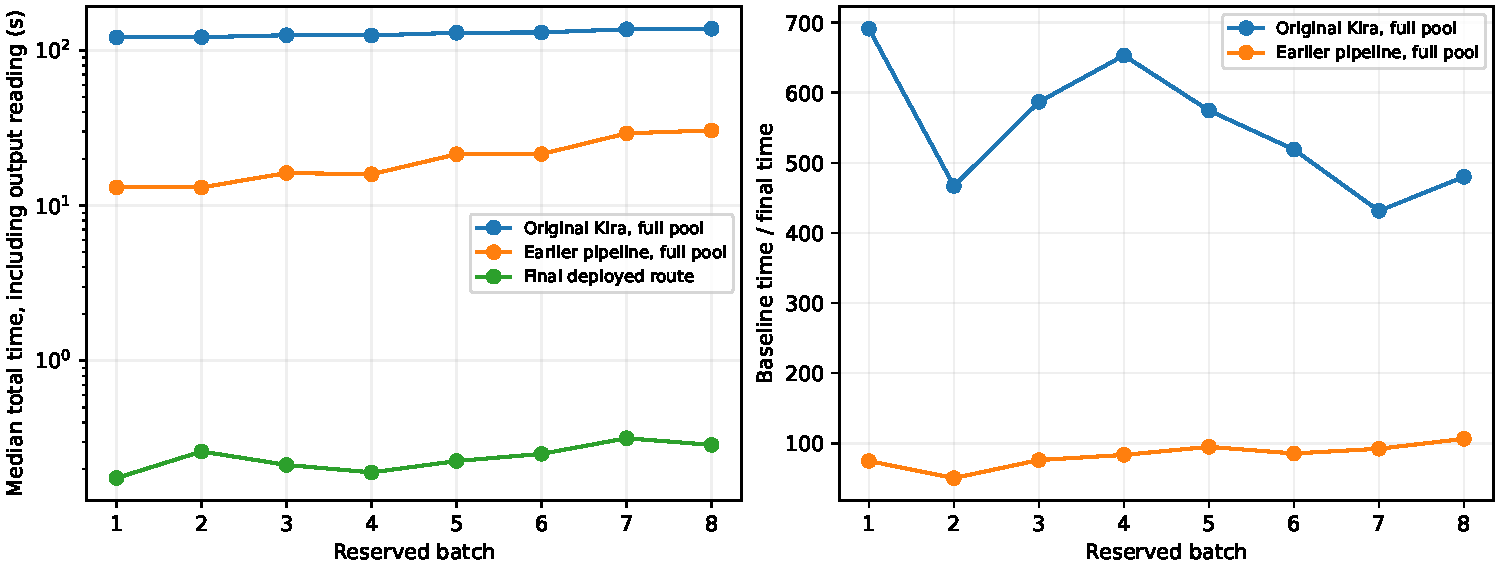
\includegraphics[width=\textwidth]{figures/cumulative_speedup.pdf}
 \caption{Direct cumulative comparison on identical reserved vacuum
 batches. The left panel shows median total times, including output
 reading, on a logarithmic scale. The right panel divides each
 baseline median by the final-route median. Each point uses five
 repetitions, three mass profiles and loop orders one through twelve.}
 \label{fig:cumulative-speedup}
\end{figure}

